\documentclass{article}
\usepackage[dblblindworkshop]{neurips_2026}
\workshoptitle{Foundation Models for Temporal Systems: From Forecasting to World Modeling}

\usepackage[utf8]{inputenc}
\usepackage[T1]{fontenc}
\usepackage{amsmath,amssymb}
\usepackage{booktabs}
\usepackage{multirow}
\usepackage{enumitem}
\usepackage{graphicx}
\usepackage{xcolor}
\usepackage{hyperref}
\usepackage{microtype}

% The style's \@trackname (which carries \workshoptitle) is only wired into the page-1
% notice under the `final' option, so a workshop *submission* otherwise renders the
% main-conference footer. Restore the workshop notice.
\makeatletter
\renewcommand{\@noticestring}{Submitted to \@trackname\ Do not distribute.}
\makeatother

% Round 11: retitled from "...Is Not a Reliable Proxy for Encoder Adaptation Benefit". The old
% subtitle equated "damage" with "adaptation benefit", which are not the same quantity -- the very
% conflation the paper argues against. This names the methodological contribution instead.
\title{Drift $\neq$ Damage: A Counterfactual Test of Encoder Adaptation in Time-Series Foundation Models}

% Double-blind: the style emits its own anonymous block and ignores \author entirely
% (neurips_2026.sty:330). Restore real names here at camera-ready.
\author{
  Anonymous Authors
}

\begin{document}

\maketitle

\begin{abstract}
% Round 12: compressed, subtraction only -- the reviewer called the opening good and the tail
% overloaded ("too much for an abstract", listing ten numbers a reader must retain). Cut: the
% +46.1% magnitude (still at Finding 3 and Table 1), the precision/recall numerals (still in the
% body and App. G -- the words "flagged all eight and only two degraded" state the same negative
% result), "so the error is systematic, not noise" (implied by "every one in the same direction"),
% and the architecture enumeration (still in Section 2). The strawman clause is softened to match
% the Introduction, and the B-D gloss now matches :101's noun phrase word for word.
Fine-tuning a time-series foundation model (TSFM) substantially changes its representations, and preservation methods exist to limit that change. But does the change tell us whether \emph{allowing} encoder adaptation was useful? We test that directly with a \textbf{frozen-encoder counterfactual}: full fine-tuning (B) against encoder-frozen adaptation (D), their difference B$-$D gated on a \textbf{pretrained-capability inclusion criterion}. \textbf{Our headline finding is methodological: B$-$D must be scored on \emph{held-out} windows.} Read on the windows model selection already uses, it flatters the frozen encoder: \textbf{selection-window bias}. Re-scored on a chronologically disjoint test split, \textbf{four of 31 cells reverse sign} (Chronos/ETTh1 $+6.8 \to -39.2$~pp), every one in the \emph{same} direction. Second, \textbf{within a backbone we find no reliable evidence that CKA magnitude predicts the held-out incremental value of allowing encoder-side adaptation} under our evaluated protocols; across three architecturally distinct TSFMs (statistically within Moirai, directionally elsewhere), two Moirai-Large $h{=}96$ cells $0.004$ apart in CKA differ by $33$~pp. Third, the intervention exposes a regime \textbf{within Moirai} we name \textbf{pretrained-capability degradation}: in eight cells meeting the criterion, full fine-tuning leaves the model \textbf{worse than not fine-tuning at all}, in every seed, while a frozen encoder \emph{improves} it. \textbf{But the criterion does not predict where}: pre-registered on eight new cells it flagged all eight and only two degraded. We establish this regime's \textbf{existence, not its prevalence}: the third backbone contains no such cell.
\end{abstract}

%% ============================================================
\section{Introduction}
\label{sec:intro}
%% ============================================================

Fine-tuning changes representations. That observation alone cannot tell us whether the change was
useful. We therefore compare full fine-tuning against an encoder-frozen counterfactual and score the
difference on \emph{held-out} data.

A Moirai encoder fine-tuned on ETTh2 can have CKA with its pretrained self fall to ${\sim}0.3$ (a ${\sim}70\%$ representational shift), and yet forecast \emph{better} on the very same task.
If drift were a proxy for damage, this should not happen.

% Round 12: softened. The old sentence asserted what practitioners *believe* -- that large drift is
% read as catastrophic forgetting -- which invites the strongest objection available against this
% paper ("nobody claims CKA is a calibrated damage metric"). The claim is now about what the
% preservation methods *do*, which the citations actually support and which App. K already says.
% The word "reflex" is retained deliberately: it is introduced here and then referred to in the box
% footer, in Finding 3's interleaving sentence, in App. D, App. F and App. K -- five sites, all of
% which still resolve against this softened antecedent. Find them with `grep -n reflex main.tex`;
% line numbers are not cited here because they shift every round.
Preservation methods such as LoRA, EWC and L2-SP~\citep{kirkpatrick2017ewc,hu2022lora,li2018l2sp} exist to limit how far fine-tuning moves a released checkpoint from its pretrained state. The \textbf{reflex} is to reach for them whenever drift is large, without first asking whether the pretrained state was worth preserving here.
This bundles three implicit claims (drift implies forgetting, forgetting implies damage, drift should be minimized), and the bundle comes apart on TSFMs. Our ``$\neq$'' is insufficiency, not independence: drift does not \emph{reliably imply} damage, because \textbf{downstream utility depends on the functional role of the changed representation}, not \emph{how much} a backbone drifts but \emph{what kind} of change it is, which one scalar cannot distinguish.

% Round 11: relocated here from Section 2, unchanged. The reviewer's most emphatic clarity ask was
% that this mental model land before the reader meets the R^2 gate, the CKA threshold, B/D and
% forgetting% -- all of which are in Section 2. It sits directly after the paragraph it answers:
% that paragraph ends on three bundled claims one scalar cannot distinguish, and these are the three
% quantities the bundle conflates. The footer line is praised by name in three consecutive review
% rounds; it must survive character-for-character.
\vspace{-1.5mm}
\begin{center}
\fbox{\begin{minipage}{\dimexpr\linewidth-2\fboxsep-2\fboxrule\relax}
\footnotesize
\textbf{Three quantities, three questions, and the paper turns on not conflating them.}\\[1.5pt]
\begin{tabular}{@{}l@{\quad}l@{\quad}l@{}}
\textbf{representation drift} (CKA) & \emph{how much changed?} & observational \\
\textbf{B$-$D} & \emph{was allowing the change worth it?} & interventional \\
\textbf{forecast MSE} & \emph{did the model improve?} & outcome \\
\end{tabular}\\[2pt]
CKA measures the first, B$-$D the second, neither is the third; \emph{damage} is what the reflex infers, not what we measure.
\end{minipage}}
\end{center}
\vspace{-1.5mm}

We contribute a within-model dissociation (Fig.~\ref{fig:dissociation}, App.~\ref{app:sweep}), a capability check across backbones with controlled encoder interventions on the cells that pass it, and a diagnostic chain needing only released weights and target data (Fig.~\ref{fig:chain}). \textbf{What is new is the combination}: a frozen-encoder counterfactual gated on \emph{demonstrated} pretrained capability, scored on held-out windows, and run on released checkpoints. On scope, \textbf{our strongest evidence comes from Moirai}: Chronos and TimesFM provide directional cross-architecture evidence, while MOMENT contributes no intervention evidence, its runs being incomplete.

Our claims, strongest evidence first. \textbf{(1) B$-$D must be scored on held-out windows}: read on the windows model selection uses, it flatters the frozen encoder, four cells reverse sign, and the gate licensing them is vulnerable the same way. \textbf{(2) Within a backbone we find no reliable evidence that CKA magnitude predicts the held-out incremental value of allowing encoder-side adaptation} under our evaluated protocols. \textbf{(3) The intervention exposes \emph{pretrained-capability degradation}}: eight Moirai cells in which full fine-tuning ends up worse than not fine-tuning at all while a frozen encoder improves on it. The downstream-only criterion that marks where capability is demonstrated is \emph{not} a validated detector of that regime, as our pre-registered arm shows.

%% ============================================================
\section{Setup and the Diagnostic Framework}
\label{sec:method}
%% ============================================================

We study four TSFMs: \textbf{Moirai}~\citep{woo2024moirai} (encoder-only, MoE), \textbf{Chronos-T5}~\citep{ansari2024chronos} (encoder--decoder), \textbf{TimesFM}~\citep{das2024timeseries} (decoder-only, $d_\text{model}{=}1280$), and \textbf{MOMENT}~\citep{goswami2024moment} (encoder-only).
Data is univariate ETT~\citep{zhou2021informer}/M4 (lookback 96; $h{=}24$ cross-backbone, $h{=}96/192$ Moirai sweep), plus ILI (weekly influenza, 7 features, lookback 104, $h{=}24$) and Electricity, \emph{restricted to 7 of its 370 series} (App.~\ref{app:crossbackbone}).
\textbf{Each arm trains through its own objective and head}; only the 5 Chronos cells attach a common MSE head to encoder states, hence limitation~(iii), and MSE magnitudes are \emph{not} comparable across arms, so B$-$D too is read within a backbone (App.~\ref{app:crossbackbone}).
Two conditions run throughout: \textbf{B}~(full fine-tuning) and \textbf{D}~(frozen encoder, head-only). Forgetting\% $= 100 (\text{MSE}_\text{FT} - \text{MSE}_\text{ZS}) / \text{MSE}_\text{ZS}$; negative means improvement over zero-shot.

\textbf{Pretrained-capability inclusion criterion.}
Before asking what adaptation is worth, we ask whether there is capability worth preserving, not whether fine-tuning is worthwhile. The check needs only released weights and the practitioner's series: does the released model beat a lookback-96 linear baseline by ${>}20\%$, that is, $R^2_\text{task} = 1 - \text{MSE}_\text{ZS} / \text{MSE}_\text{Linear} \geq 0.20$?
\textbf{Its role is inclusion, not prescription: it decides which cells make an intervention interpretable, and is \emph{not} a validated deployment-time decision rule.}

\textbf{CKA drift.}
Linear CKA~\citep{kornblith2019cka} between pretrained and fine-tuned backbone on mean-pooled encoder outputs over identical held-out 192-timestep windows; flagged at $<0.95$ and compared only \emph{within} a backbone, never across architectures. CKA remains a valid similarity measure; our claim is only that its magnitude should not be read as downstream damage.
Pooling moves the CKA magnitude but not the flag (App.~\ref{app:thresholds},~\ref{app:pooling}).

\textbf{Frozen-encoder intervention (B$-$D).}
Condition D measures what head-only training achieves when the encoder cannot move; B$-$D is the resulting forgetting\% gap in percentage points, negative meaning adaptation helps. Freezing applies to encoder weights only (input/output projections stay trainable), so D is not representation-frozen (CKA $0.38$--$1.000$). \textbf{B$-$D therefore estimates the \emph{incremental downstream value of allowing encoder-side adaptation} under this training protocol, not the causal effect of the representation change CKA measures.} Freezing also removes optimization degrees of freedom, so no single mechanism is isolated by this contrast.

\begin{figure}[t]
\centering
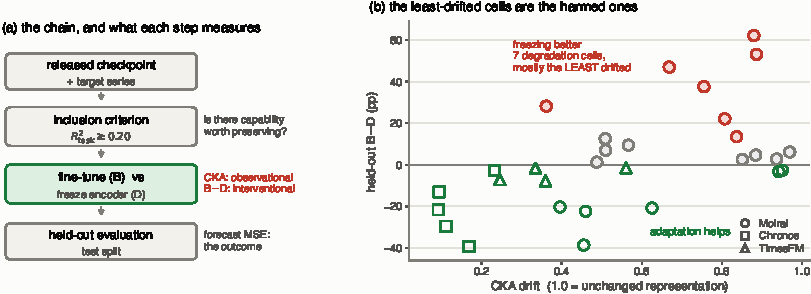
\includegraphics[width=\linewidth]{../fig1_diagnostic_flow.pdf}
\vspace{-5mm}
% Round 12: trimmed. The reviewer's density complaint about page 3 was that "the prose should do
% less work" -- and each panel's own in-figure title already states its claim ("the intervention
% answers what drift cannot", "no cut on CKA separates the two regimes"), which this caption was
% restating. Both restatements are gone; the 4-of-31 fact and the 0.622/0.626 pair stay.
\caption{\textbf{Drift cannot stand in for the intervention.}
\textbf{(a)}~The last step must be asked on held-out windows: scored on the selection split
instead, four of 31 cells come out with the \emph{opposite} sign, every one flattering the frozen
encoder. \textbf{(b)}~All 31 cells; red marks the eight \textbf{pretrained-capability degradation}
cells, and the two Moirai-Large $h{=}96$ cells at CKA $0.622$/$0.626$ fall on opposite sides of the
regime; the $x$-axis is not a decision boundary (App.~\ref{app:crosscell}).}
\label{fig:chain}
\end{figure}

%% ============================================================
\section{Results: Three Findings}
\label{sec:results}
%% ============================================================

Table~\ref{tab:regimes} summarizes the cross-backbone results, ordered by B$-$D; pretrained value proves to be a property of checkpoint $\times$ dataset $\times$ horizon rather than of an architecture (App.~\ref{app:crossbackbone}).

% Round 11: permuted to claim -> why -> evidence -> caveat (Findings 2 and 3 already read that way),
% and the two split terms are defined here once so the body can stop alternating between
% "evaluation windows", "validation" and "out of sample". The closing caveat sentence is
% reviewer-protected in two rounds and is unchanged.
\textbf{Finding 1 (methodological): B$-$D must be scored on held-out windows.}
Two splits, used throughout: the \textbf{selection split} trains the models and chooses among them, and the \textbf{test split} is chronologically disjoint and used for neither. \textbf{B$-$D read on the selection split estimates no generalization quantity, and its \emph{sign} is not safe there}: \textbf{selection-window bias}. The reason is that B$-$D compares two trained models and inherits the model selection of both: B early-stops on the selection split and a frozen head's regularizer is tuned there, so both arms are tuned on the windows the difference is then read on, and nothing constrains them to profit from that equally. Re-scored on the test split, \textbf{four of the 31 cells reverse sign} (Chronos/ETTh1 largest at $+6.8{\pm}2.9 \to -39.2{\pm}13.9$, joined by both Moirai/ETTh2 cells and TimesFM/ETTh2, whose $+0.2{\pm}2.9$ leaves it the least informative of the four), while others merely soften, and all four run the same way: on the selection split, B$-$D \emph{flatters the frozen encoder}. We cannot separate selection overfitting from validation-to-test shift (the \emph{untrained} model's own error differs up to fivefold between the two window sets), so this is a protocol-level failure, not a mechanism (App.~\ref{app:heldout}). The prescription is unsurprising; that ignoring it inverts 4 of 31 conclusions, by up to $46$~pp and always in the same direction, is not.

\textbf{The criterion says where the question is meaningful, not where fine-tuning will fail.}
The gate inherits selection the same way, and the eight cells below were identified \emph{retrospectively}, so we \textbf{pre-registered} the criterion on eight new cells, committed to git before any run. It \textbf{flagged all eight; two degraded}: \textbf{precision $0.25$ at recall $1.00$}. The gate defines the population in which the counterfactual question is meaningful; our prospective experiment gives no evidence that it can identify degradation.

\textbf{Finding 2: drift magnitude does not order the intervention.}
Sharpest is a near-tie: two Moirai-\emph{Large} $h{=}96$ cells at CKA $0.622$/$0.626$ sit at B$-$D
${+}12.0$/${-}20.8$~pp, same backbone, size and horizon, $33$~pp apart, and no cut separates them.
Nor is there reliable evidence that CKA \emph{orders} the held-out column \emph{within} a
backbone: $\rho{=}+0.168$ over 22 Moirai cells, on a CI wide enough to leave a moderate positive
effect open, and the slope stays unpinned when backbone identity is absorbed as a fixed effect
($n{=}31$, App.~\ref{app:crosscell}). This is evidence of \textbf{non-reliability} under the evaluated
protocols, not proof of zero association.

% Round 12: the table's SOURCE position moved here, from just after the paragraph that introduces it.
% Nothing about the table itself changed. This is the reviewer's page-3 complaint -- "the figure, the
% table and the prose are all competing for attention" -- and it was a float-placement artefact: a [t]
% float is eligible for the top of the page it is DECLARED on, so while it was declared early it kept
% landing on page 3 beside Fig. 1. It has to be declared past where page 3 breaks, which is inside
% Finding 3; declared here it lands at the top of page 4. Page 3 now carries one visual and page 4 the
% other. Two earlier positions were tried and both still put it on page 3 -- do not move it back
% without re-running the per-page float probe.
%   for p in 3 4; do pdftotext -f $p -l $p main.pdf - | grep -c 'Backbone'; done   # want 0 then 1
\begin{table}[t]
\centering
\caption{\textbf{Does CKA tell us whether freezing helps? No: the CKA column does not order the
B$-$D column.} Held-out B$-$D (pp): ${<}0$ \textbf{adaptation helps}, $\mathbf{>0}$ \textbf{freezing
helps}. 31 cells, 3--10 seeds, scored on test. $^{\text{f}}$gate-fails; $^{*}|$mean$|<2$\,SEM;
$^{\ddagger}$B$-$D only (limitation~iii); $^{\text{p}}$pre-registered. Per-cell gate values and
B$-$D App.~\ref{app:heldout}; statistics App.~\ref{app:crosscell}.}
\label{tab:regimes}
% \small overflows \textwidth by 27pt on the Chronos row; the air comes from \arraystretch and the
% removed negative \vspace instead. Gate R^2 values were dropped from column 2 in round 10 -- they
% answer a different question than the table's one question, and heldout_all.tex carries them all.
\footnotesize
\setlength{\tabcolsep}{3pt}
\renewcommand{\arraystretch}{1.0}
\begin{tabular}{@{}llccl@{}}
\toprule
Backbone & Data ($h$) & CKA & B$-$D held-out & Reading \\
\midrule
Chronos$^{\ddagger}$  & ETTh1, ETTm2, Weather, ETTh2, Elec.$^{\text{f}}$ (24) & 0.09--0.23 & $-39.2$ to $-2.7^{*}$ & adapt \\
Moirai-S & ILI (24)$^{\text{f}}$ & 0.455 & $-38.6$ & adapt \\
Moirai-B & ETTh2 (96 / 192) & 0.40--0.46 & $-22.3$ / $-20.2$ & adapt \\
Moirai-L & ETTh2 (96)$^{\text{f}}$ & 0.626 & $-20.8$ & adapt \\
TimesFM  & ETTm2, ETTh2, Weather, ETTh1 (24) & 0.25--0.56 & $-7.7$ to $-1.4^{*}$ & adapt \\
Moirai-S$^{\text{p}}$ & Electricity (96 / 192) & 0.94--0.95 & $-3.2$ / $-2.6^{*}$ & adapt \\
% Round 11: +6.2 -> +6.1. The row's largest cell is Moirai-Small/ETTh2 h192 n500 at +6.1482, which
% App. L's generated table already prints as $+6.1{\pm}3.4$; the typo made Table 1 disagree with it.
Moirai-S & ETTh2, ETTm2 (96 / 192) & 0.85--0.97 & $+2.6$ to $+6.1^{*}$ & freeze \\
Moirai-B$^{\text{p}}$ & ETTm2, Weather (96 / 192) & 0.49--0.57 & $+1.3^{*}$ to $+12.5^{*}$ & freeze \\
Moirai-L$^{\text{p}}$ & Weather (96) & 0.622 & $\mathbf{+12.0}^{*}$ & \textbf{degradation} \\
Moirai-S, L$^{\text{p}}$ & ETTh1 (96 / 192) & 0.36--0.84 & $\mathbf{+13.5}$ to $\mathbf{+28.2}$ & \textbf{degradation} \\
Moirai-B & ETTh1 (96 / 192) & 0.67--0.76 & $\mathbf{+37.5}$ / $\mathbf{+47.0}$ & \textbf{degradation} \\
Moirai-S & Weather (96 / 192) & 0.88--0.89 & $\mathbf{+53.1}$ / $\mathbf{+62.1}$ & \textbf{degradation} \\
\bottomrule
\end{tabular}
\vspace{-4mm}
\end{table}

\textbf{Finding 3: fine-tuning can leave the model worse than not fine-tuning at all.}
In eight Moirai cells, full encoder fine-tuning \emph{destroys} the pretrained advantage the
criterion demonstrated, while freezing the encoder keeps it, so the practitioner would have been
better off leaving the checkpoint alone. We name this regime \textbf{pretrained-capability
degradation} and define it \textbf{empirically} by three clauses, the last two required in
\emph{every} seed: the cell gate-passes, B ends up worse than the un-tuned model, and D improves
on it. Moirai-Small/Weather is clearest: B lands $+37.3\%$/$+46.1\%$ \emph{above}
zero-shot error while D reaches $-15.8\%$/$-16.0\%$. \textbf{On ETTh1 it holds at all three released sizes} (Large prospectively, $+14.1\%$ under B against
$-14.1\%$ under D, 3/3); on Weather it is present at Small and again at Large but absent at Base, so
neither dataset nor size predicts it alone. Nor does drift flag them: the eight span CKA
$0.36$--$0.89$ while the seven cells adaptation helps by ${\ge}20$~pp span $0.09$--$0.63$, so the
bands \textbf{interleave} and the reflex would have cleared damaging cells and flagged safe ones.

\textbf{Robustness.} Freezing the input projections too (condition~H, CKA exactly $1.0$) keeps B$-$D's
sign on all seven cells run (six of the eight degradation cells, plus ILI), so ``freezing helps'' is
not input re-fitting (App.~\ref{app:strictfreeze}).
\textbf{A third backbone.} TimesFM-2.5 under its \emph{own} recipe (no head attached, so both
forgetting\% terms are clean) gate-passes on four datasets and \textbf{none is a degradation cell}: B
beats zero-shot in all four, B$-$D running $-7.7$ to $-1.4$ (scope, not generality).
\textbf{Representation similarity is not a property of the backbone weights alone.} In condition~D
TimesFM's transformer stack is \textbf{bit-identical} after
training ($\ell_2$ drift exactly $0.00$) yet reads CKA $0.38$--$0.89$, all of it the input tokenizer, so
low CKA cannot by itself mean a damaged encoder (App.~\ref{app:crossbackbone}).

%% ============================================================
\section{Discussion}
\label{sec:discussion}
%% ============================================================

\textbf{What this is and is not.} The sign reversals are a generalization result: no model is fitted
or selected on test. The degradation regime is \emph{identified} using test data, so it establishes
existence, not prevalence; the pre-registered arm bounds its detection accuracy
(App.~\ref{app:heldout}). Runs were not blinded and two pre-specified predictions were falsified.

\textbf{The one sentence to carry away.} For TSFM adaptation, representation drift is an
\emph{observational diagnostic}, not a substitute for the counterfactual question of whether
\emph{allowing} encoder adaptation improves held-out utility.

% Round 11: the same three-item rule that used to run inline above, boxed. The reviewer's ask was to
% make the operational rule visually isolated and memorable; the sentence above stays because it is
% the conceptual claim and the box is the procedure. Same stock \fbox+minipage as the Section 1 box
% -- no box package is loaded, do not add one.
\vspace{-1mm}
\begin{center}
\fbox{\begin{minipage}{\dimexpr\linewidth-2\fboxsep-2\fboxrule\relax}
\footnotesize
\textbf{Practical takeaway: do not infer damage from drift.}\\[1.5pt]
\textbf{1. Check capability.} Does the released checkpoint beat a lookback-96 linear baseline?\\
\textbf{2. Test adaptation.} Compare full fine-tuning against a frozen encoder.\\
\textbf{3. Use held-out data.} Score B$-$D only on a chronologically disjoint test split.
\end{minipage}}
\end{center}
\vspace{-1mm}

Scripts, per-seed run records and the
pre-registration (committed before any run) will be released with the paper.

\textbf{Limitations} (related work App.~\ref{app:related}). \emph{(i)} Two analyses from an earlier version are \textbf{withdrawn}, sharing no machinery with B$-$D (App.~\ref{app:probes},~\ref{app:crosscell}). \emph{(ii)} Cells are unequally powered and \textbf{not independent}, so cross-cell statistics are descriptive. \emph{(iii)} Chronos carries no per-condition forgetting\% ($\ddagger$, Table~\ref{tab:regimes}); the degradation cells are Moirai-only. \emph{(iv)} Condition~D leaves input projections trainable, and the strict-freeze control (App.~\ref{app:strictfreeze}) covers six of the eight cells: five keep both parts of the degradation definition, but on Moirai-Small/ETTh1 $h{=}192$ the strictly-frozen model no longer beats the un-tuned one.

\bibliographystyle{plainnat}
\bibliography{workshop_refs}

\appendix

%% ============================================================
\section{Within-Model Dissociation Sweep}
\label{app:sweep}
%% ============================================================

Every point shares a backbone, a dataset, a horizon and a protocol; only the fine-tuning sample size
varies. Increasing $n$ moves drift monotonically while the task outcome moves non-monotonically:
CKA falls steadily from $0.949$ at
$n{=}500$ to $0.518$ at $n{=}10$k, while forgetting goes $+14.0$, $+13.4$, $-2.9$, $+6.6$,
$-5.3\%$. The best cell in the sweep is the \emph{most}-drifted one.
The $n{=}5$k variance ($+6.6\%$, std $10.0$, 7 seeds) is bimodal: 4 seeds near $-0.1\%$, 3 at
$+15.5\%$ with an epoch-1 overshoot, so we treat that point as unresolved rather than as evidence
for either direction.

This is a \emph{dissociation, not an intervention on drift.} Sample size is an uncontrolled causal
variable: raising it changes supervision, optimization trajectory and overfitting, not drift alone.
The sweep therefore shows that drift and outcome need not move together within one model; it cannot
show that drift itself is causally inert. The frozen-encoder experiment is the intervention, and it
is what the paper's claims rest on.

\begin{figure}[h]
\centering
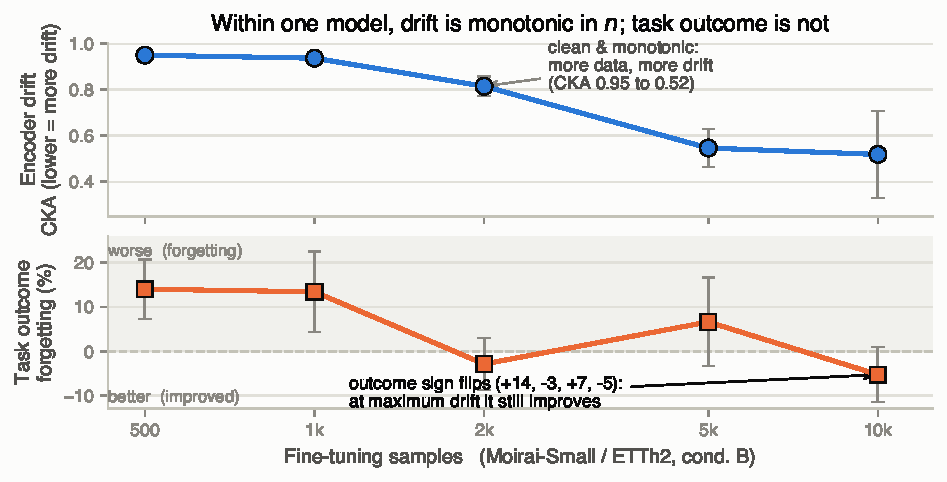
\includegraphics[width=\linewidth]{../fig2_dissociation_sweep.pdf}
\vspace{-4mm}
\caption{\textbf{Within-model dissociation.}
Moirai-Small/ETTh2 ($h{=}96$, cond.~B) across $n$: as $n$ rises CKA drift is monotonic (top) while forgetting is non-monotonic and sign-flipping (bottom), improving at maximum drift: \textbf{drift and downstream outcome can move independently}. Sample size is uncontrolled here, so this demonstrates \textbf{non-monotonic co-movement, not causal independence}: it is a dissociation, not an intervention on drift.
Error bars $\pm 1$ SD; $n{=}10$k is 10-seed CUDA-deterministic.}
\label{fig:dissociation}
\end{figure}

%% ============================================================
\section{The Retracted Probe Analysis}
\label{app:probes}
%% ============================================================

We initially used a linear-probe analysis. We reproduced the published statistic but found that it
depended on a non-generalizing probe ($R^2 \approx -6.9$) and disappeared under a protocol in which
the probe generalizes. We therefore \textbf{retract this analysis}. It shares no data-processing
machinery with the frozen-encoder intervention, which manipulates the encoder rather than fitting a
readout on it and is measured in forecast MSE rather than $R^2$; the reversals in
\S\ref{sec:results} were never probe-dependent. The numbers are kept here, unchanged, so the
retraction can be audited.

\textbf{What was published, and that it reproduces.} On Moirai-Small/ETTh2 ($h{=}96$, $n{=}10$k) the
trained 96-step probe gave $\Delta R^2 = +0.67{\pm}0.23$ (10/10 seeds positive) while four auxiliary
probes decreased: mean $-0.033{\pm}0.019$ (10/10 neg), variance $-0.048{\pm}0.030$ (9/10),
lag-1 autocorrelation $-0.052{\pm}0.041$ (9/10), GBM delta1 $-0.056{\pm}0.030$ (4 seeds), and
forecast-48 was indistinguishable from zero ($-0.001{\pm}0.163$, 4 seeds). Classification used an
effect-size heuristic, whether the mean exceeds one seed-level SD, not a significance test. The five
targets vary along two axes a single probe family would confound: \emph{what} is decoded (low-order
statistics vs.\ forecasts) and \emph{how} (linear Ridge vs.\ gradient-boosted). The pipeline was not
documented in enough detail to re-run, so we recovered it from source: encoder input of \textbf{192}
steps (lookback $+$ horizon), probe trained on the first 300 validation windows and evaluated on the
first 200 test windows, target the next 96 steps across all seven features flattened,
Ridge($\alpha{=}1.0$) on mean-pooled outputs. That reproduces the published values to four
significant figures: $R^2(\text{PT}){=}-6.9043$ (published $-6.90$), $R^2(\text{FT}){=}-6.2364$
($-6.23$), $\Delta R^2{=}+0.6679{\pm}0.2262$ ($+0.67{\pm}0.23$), 0/10 negative. Three details each
move the result by an order of magnitude: the 192-step window rather than a 96-step context,
evaluating across the validation$\rightarrow$test boundary rather than within one split, and using all
seven features rather than the target channel alone; a within-validation split moves
$R^2(\text{PT})$ from $-6.90$ to $-0.13$.

\textbf{A protocol with every knob fixed in advance} (\texttt{scripts/probe\_transparent.py}): the
same 500 windows; mean-pooled encoder output standardized on probe-train; Ridge with $\alpha$ chosen
by 5-fold CV on the \emph{pretrained} encoder's probe-train over $\log_{10}\alpha \in [-3, 6]$ and
then reused for all ten fine-tuned encoders, so the two are never tuned apart; $\Delta R^2$ per seed
with a percentile bootstrap 95\% CI over the ten seeds (10{,}000 resamples). Two additions decide the
outcome: \textbf{two splits} ($T$, the published temporal split, and $R$, the same 500 windows
randomized into 300/200), which separates decodability from the validation$\rightarrow$test level
shift, and a \textbf{permuted-target noise floor}, the identical pipeline run on 20 independently
shuffled copies of each target, so a real $\Delta R^2$ must exceed what the pipeline produces when the
target carries no information at all.

\begin{table}[h]
\centering
\caption{Transparent protocol, Moirai-Small/ETTh2, 10 released checkpoints. Under the published
split $T$ \emph{no probe generalizes} ($R^2(\text{PT}){<}0$) and every $|\Delta R^2|$ is far
below the permuted-target floor. Under $R$, where every probe generalizes, no $|\Delta R^2|$
exceeds $0.011$ and the trained probe \emph{decreases}.}
\label{tab:transparent}
\small
\begin{tabular}{@{}llrrr r@{}}
\toprule
Split & Target & $R^2(\text{PT})$ & $\Delta R^2$ & 95\% CI & floor \\
\midrule
\multirow{4}{*}{$T$}
 & Forecast-96 (trained) & $-5.23$   & $-0.0005$ & $[-0.001, +0.000]$ & $0.0005$ \\
 & Mean                  & $-164.09$ & $+3.22$   & $[-3.60, +10.00]$  & $102.1$ \\
 & Variance              & $-20.50$  & $-8.22$   & $[-11.94, -4.14]$  & $132.3$ \\
 & Lag-1 autocorr.       & $-2.71$   & $-0.80$   & $[-2.02, +0.16]$   & $30.7$ \\
\midrule
\multirow{4}{*}{$R$}
 & Forecast-96 (trained) & $+0.678$ & $-0.0042$ & $[-0.0061, -0.0025]$ & $0.019$ \\
 & Mean                  & $+0.994$ & $-0.0014$ & $[-0.0022, -0.0006]$ & $0.226$ \\
 & Variance              & $+0.937$ & $+0.0025$ & $[-0.0014, +0.0068]$ & $0.169$ \\
 & Lag-1 autocorr.       & $+0.750$ & $+0.0103$ & $[+0.0012, +0.0194]$ & $0.223$ \\
\bottomrule
\end{tabular}
\end{table}

\textbf{The effect is a regularization artifact.} Holding the split at $T$ and sweeping $\alpha$, the
trained probe's $\Delta R^2$ decays monotonically: $+0.668$, $+0.271$, $+0.066$, $+0.034$, $+0.005$,
$+0.000$ at $\alpha = 1, 10, 10^2, 10^3, 10^4, 10^5$, while $R^2(\text{PT})$ stays between $-6.90$
and $-5.23$. It is largest exactly where the probe extrapolates worst, and CV on the training split
selects $\alpha{=}10^6$, at which it vanishes. Under $R$, where the trained probe attains
$R^2(\text{PT}){=}+0.68$, $\Delta R^2$ is at most $+0.017$ at any $\alpha$ and is negative at the
CV-selected value. No configuration has the trained probe both generalizing and increasing by
anything near $+0.67$. Target normalization is provably not a knob: with an intercept, Ridge is
equivariant under affine target scaling, and the sweep confirms the rows are identical to the last
digit. The criterion that disqualified the Ridge delta1 probe was that its zero-shot
baseline is negative enough ($R^2 \approx -2.3$) that any encoder shift inflates $\Delta R^2$, which
is why we reported the GBM version on a genuine positive floor ($R^2(\text{PT}){=}{+}0.059$, on which
decodability \emph{falls}) rather than Ridge's $+1.04{\pm}0.22$. Applied consistently, that criterion
disqualifies the headline trained probe at $-6.90$ as well.

\textbf{What survives.} Under the one split where all seven probes generalize, every $|\Delta R^2|$
is $\le 0.011$: the trained probe \emph{decreases} ($-0.0042$, 10/10 seeds), mean and trend decrease,
lag-1 autocorrelation \emph{increases}, and variance, lag-24 and spectral centroid are
indistinguishable from zero. That is not the claimed asymmetry; it is closer to no detectable change
in any direction. Five probes could not have established the absence of specialization along an
unmeasured axis (calibration, periodicity, tail behaviour) in any case, and the GBM delta1 probe was
the only positive-floor untrained readout available to us.

%% ============================================================
\section{ILI Cell Detail}
\label{app:ili}
%% ============================================================

\textbf{ILI gate-fails on held-out windows.}
Computed from the runs this paper reports (10 seeds, \texttt{results/v40\_ili\_heldout}), the gate is
$+0.139$ on validation (ZS $1.893$, linear $2.206$) and $\mathbf{-0.033}$ on the test segment
(ZS $2.479$, linear $2.664$); an earlier gate-pass figure is withdrawn. The per-feature picture is why the mean lands where it does: five of seven features are
positive but only two clear $0.20$, and \textsc{num.\ of providers} is $-0.86$ because that series is
close to a straight line on the test segment, which linear extrapolation fits almost exactly. ILI is
not a degradation cell and no claim in \S\ref{sec:results} rests on its gate; what changes is that it
can no longer be cited as a moderate-gate cell, and the ``falsified prediction'' below is
correspondingly weaker evidence: a heavily restructuring encoder on a cell with \emph{no}
demonstrated zero-shot advantage is much less surprising than one on a moderate-gate cell.

\textbf{Status of this cell.}
On ILI the encoder restructures heavily (CKA $0.455{\pm}0.008$) and full fine-tuning improves by $-80.0{\pm}0.6\%$ (10/10), falsifying a prediction specified beforehand ($0.90$--$0.95$ CKA expected). We previously reported B$-$D${=}{-}80.7$~pp here, i.e.\ that encoder adaptation supplied \emph{all} of the gain. That is withdrawn. The frozen control it was measured against had never been trained: the script assigned the zero-shot MSE as the fine-tuned MSE and wrote a forgetting of exactly $0.0$, so the ``$0.0\%$ in all 10 seeds'' was one constant, not ten measurements. Re-run so that condition~D actually trains (encoder frozen, the $3.2$M parameters outside it updated), the gap is $-62.6{\pm}1.4$ on validation and $-38.6{\pm}1.3$ held-out (10/10 negative on both). D reaches CKA $0.76$--$0.90$, not $1.000$, because the projections feeding the encoder remain trainable. Condition~B is unaffected and reproduces the published $-80.7{\pm}0.9$ and CKA $0.478$ to within seed noise, so the entire discrepancy was the untrained control. Note also that both references are weak in absolute terms (ZS MSE $1.893$, linear $2.206$ on validation).


The cell is Moirai-Small on national influenza-like illness: 966 weekly observations, 7 features,
$h{=}24$, lookback 104, split 579/193/194 chronologically.
Condition~D, re-run so that it trains, gives CKA $0.827{\pm}0.013$ and forgetting $-17.4{\pm}1.3\%$ on validation ($-12.2{\pm}1.3\%$ held-out), 10/10 negative: head-only training recovers a substantial share of the improvement, so the B$-$D gap is $-62.6$~pp on validation and $-38.6$~pp held-out, not the $-80.7$ previously reported.

\begin{table}[h]
\centering
\caption{ILI per-seed results (Moirai-Small, $h{=}24$, lookback 104), both conditions,
regenerated for this revision. Each value is the mean across the 7 univariate features.
The $\Delta R^2$ column of the earlier version of this table is dropped with the retracted probe
axis; condition~D is shown because it previously did not exist as a measurement.}
\label{tab:iliperseed}
\small
\begin{tabular}{@{}lccc@{}}
\toprule
 & \multicolumn{2}{c}{B (full fine-tuning)} & D (frozen encoder) \\
\cmidrule(lr){2-3}\cmidrule(lr){4-4}
Seed & CKA & Forg.\% (val / held-out) & CKA \quad Forg.\% (val / held-out) \\
\midrule
42  & 0.458 & $-78.6$ / $-51.5$ & 0.804 \quad $-16.2$ / $-14.6$ \\
101 & 0.465 & $-81.4$ / $-50.1$ & 0.898 \quad $-13.5$ / $-6.7$ \\
123 & 0.476 & $-80.0$ / $-48.9$ & 0.756 \quad $-27.6$ / $-19.5$ \\
202 & 0.457 & $-81.4$ / $-52.1$ & 0.791 \quad $-19.7$ / $-13.6$ \\
303 & 0.409 & $-78.1$ / $-49.0$ & 0.823 \quad $-18.3$ / $-11.5$ \\
456 & 0.463 & $-75.5$ / $-50.0$ & 0.851 \quad $-15.4$ / $-13.2$ \\
777 & 0.437 & $-81.6$ / $-52.5$ & 0.822 \quad $-18.0$ / $-12.4$ \\
789 & 0.449 & $-80.3$ / $-49.5$ & 0.865 \quad $-12.7$ / $-4.9$ \\
888 & 0.505 & $-82.0$ / $-50.8$ & 0.848 \quad $-16.1$ / $-12.8$ \\
999 & 0.437 & $-80.8$ / $-53.4$ & 0.807 \quad $-16.1$ / $-12.7$ \\
\midrule
Mean & 0.456 & $-80.0$ / $-50.8$ & 0.827 \quad $-17.4$ / $-12.2$ \\
\bottomrule
\end{tabular}
\end{table}

\textbf{Per-feature asymmetry.}
The forecast target OT shows the largest gain ($+0.73{\pm}0.16$, 10/10 positive) and AGE~0--4 also gains consistently ($+0.15{\pm}0.05$, 10/10).
AGE~5--24 is negative ($-0.07{\pm}0.09$, 3/10 positive).
Decodability thus improves on the target and degrades on a series the head was not optimizing, the same signature as the ETTh2 trained-vs-auxiliary split, obtained here within a single cell.

\textbf{Falsified prediction.}
We specified CKA $0.90$--$0.95$ for ILI in advance, on the expectation that a moderate gate implies moderate drift.
The observed $0.456$ falsifies this: gate strength does not linearly predict drift magnitude, and the restructuring-to-stability transition sits nearer ${\approx}80\%$ gate than the $50$--$70\%$ we assumed.
We report this because it is the kind of prediction the chain is supposed to expose.

%% ============================================================
\section{Full Preservation Spectrum}
\label{app:preservation}
%% ============================================================

\textbf{What this appendix is for.} It is a \emph{secondary}, observational result: it shows that
raising representational similarity does not raise utility, which is evidence against the reflex's
prescriptive half. It is \textbf{not} evidence for this paper's interventional claim; that rests entirely on
the frozen-encoder intervention B$-$D in \S\ref{sec:results}, because these methods preserve
representations by different mechanisms and so are not a controlled manipulation of one variable.
The main text quotes $h{=}96$ only.
Table~\ref{tab:mitigation_spectrum} gives both horizons and all methods, including the NLL+SupCon variant.
These methods preserve representations by \emph{different mechanisms}, namely penalty (L2-SP, EWC), reparameterization (LoRA), and complete freezing, so CKA is a common observational axis, not a common intervention, and at $n{=}4$--$7$ the correlations here are descriptive only. We stress that \textbf{LoRA does well}: the paper's claim is that drift magnitude fails to \emph{order} these methods, not that preservation is a bad idea or that fine-tuning should be avoided.
\textbf{The matched spectrum} puts every method
at $n{=}1000$, $h{=}96$, each run against its own zero-shot: full fine-tuning is CKA $.936$ at
$+13.4\%$, against L2-SP $\lambda{=}0.01$ ($.939$, $+16.0$), L2-SP $\lambda{=}0.1$ ($.965$, $+13.4$),
EWC $\lambda{=}1000$ ($.972$, $+14.9$) and LoRA ($.979$, $-9.2$).

The claim this displaces is the strong one: it is \emph{not} true that every weight-anchoring
configuration forecasts worse. L2-SP $\lambda{=}0.1$ raises CKA substantially ($.936 \to .965$) and
lands on full fine-tuning to within $0.02$~pp. What the corrected spectrum shows is the weaker and
more useful thing, that moving up the CKA axis buys nothing predictable: one anchoring setting is worse,
one is a dead heat, a third is worse again, and the reparameterizing method is far better while
being the most CKA-preserving of the four. Representation preservation does not predict utility
here. At $h{=}192$ no $n{=}1000$ full-fine-tuning baseline exists in our runs, so we report that
horizon's methods without a matched reference rather than against the $n{=}500$ one.

% GENERATED by scripts/emit_mitigation_spectrum.py -- do not edit by hand.
\begin{table}[t]
\centering
\caption{\textbf{Mitigation spectrum on Moirai-Small/ETTh2.}
Rows ordered by representation preservation (CKA at $h{=}96$).
On \emph{this} cell LoRA preserves representations (CKA${\approx}0.98$) while
\emph{improving} on zero-shot, and weight anchoring reduces drift without buying
utility.  \textbf{Neither reading generalises, and we checked rather than assumed:}
extending condition~E to 8 further value-cells
(Appendix~\ref{app:loravaluecells}) puts CKA$_\text{E}$ anywhere from $0.55$ to
$0.97$ and leaves full fine-tuning ahead of LoRA on 4 of the 8.
\textbf{Every row is scored against its own zero-shot.} Forgetting\% is the
mean over seeds of each run's $(\text{fine-tuned}-\text{zero-shot})/
\text{zero-shot}$, so no row borrows another's denominator; earlier versions of
this table divided the anchoring and LoRA rows by a single shared value and read
up to $3.4$~pp away as a result.  MSE, CKA and $\ell_2$ drift are means over
seeds with population std (ddof${=}0$); the body's SEM convention
(\S\ref{sec:method}) does not apply here.
\textbf{The rows are not matched on training-set size.}
Conditions B, C and D use $n{=}500$ training samples (zero-shot MSE $.1256$ at $h{=}96$, $.1580$ at $h{=}192$);
E, F and G use $n{=}1{,}000$ (zero-shot MSE $.1274$ and $.1596$); the two rightmost
columns give the seed count and the training-set size separately.
We therefore claim no ordering \emph{between} the two
groups: there is no full-fine-tuning arm at $n{=}1{,}000$ on this cell with more
than a single seed, so ``anchoring ties full fine-tuning'' is not a comparison
these runs support.  The dissociation the table is cited for (CKA not predicting
utility) is within-group and unaffected.
Condition~D reads CKA $0.99996$ rather than $1$: it leaves \texttt{in\_proj} and
\texttt{mask\_encoding} trainable, so it is a frozen-\emph{encoder} control and not
a strict freeze.  Only condition~H (Appendix~\ref{app:strictfreeze}) is $1.0000$ by
construction.  Earlier versions of this table printed D as $1.000$, which rounded
that distinction away.}
\label{tab:mitigation_spectrum}
\small
\resizebox{\textwidth}{!}{%
\begin{tabular}{l cccc cccc cc}
\toprule
& \multicolumn{4}{c}{$h=96$} & \multicolumn{4}{c}{$h=192$} & & \\
\cmidrule(lr){2-5} \cmidrule(lr){6-9}
Method & MSE & Forg.\% & CKA & Drift & MSE & Forg.\% & CKA & Drift & seeds & $n$ \\
\midrule
B: Full fine-tune & .140{\tiny$\pm$.014} & $+$11.1 & .937{\tiny$\pm$.028} & 3.96{\tiny$\pm$.56} & .183{\tiny$\pm$.020} & $+$15.7 & .970{\tiny$\pm$.009} & 4.12{\tiny$\pm$.32} & 10 & 500 \\
F: L2-SP ($\lambda{=}0.01$) & .150{\tiny$\pm$.006} & $+$16.0 & .939{\tiny$\pm$.023} & 4.98{\tiny$\pm$.34} & .179{\tiny$\pm$.009} & $+$12.7 & .945{\tiny$\pm$.007} & 4.84{\tiny$\pm$.22} & 3 & 1{,}000 \\
C: NLL+SupCon & .138{\tiny$\pm$.010} & $+$10.1 & .949{\tiny$\pm$.014} & 3.72{\tiny$\pm$.43} & .178{\tiny$\pm$.011} & $+$12.9 & .964{\tiny$\pm$.015} & 3.97{\tiny$\pm$.34} & 10 & 500 \\
F: L2-SP ($\lambda{=}0.1$) & .147{\tiny$\pm$.003} & $+$13.4 & .965{\tiny$\pm$.006} & 2.94{\tiny$\pm$.08} & .181{\tiny$\pm$.003} & $+$13.6 & .980{\tiny$\pm$.002} & 2.84{\tiny$\pm$.02} & 3 & 1{,}000 \\
G: EWC ($\lambda{=}1000$) & .149{\tiny$\pm$.015} & $+$14.9 & .972{\tiny$\pm$.004} & 3.29{\tiny$\pm$.79} & .188{\tiny$\pm$.004} & $+$18.3 & .978{\tiny$\pm$.006} & 4.46{\tiny$\pm$.38} & 3 & 1{,}000 \\
E: LoRA ($r{=}8$)\textsuperscript{$\dagger$} & \textbf{.116}{\tiny$\pm$.001} & \textbf{$-$9.1} & .979{\tiny$\pm$.006} & 0.00{\tiny$\pm$.00} & \textbf{.157}{\tiny$\pm$.002} & \textbf{$-$1.8} & .986{\tiny$\pm$.005} & 0.00{\tiny$\pm$.00} & 5 & 1{,}000 \\
\midrule
D: Frozen encoder & .126{\tiny$\pm$.006} & $+$0.5 & .99996{\tiny$\pm$.00001} & 1.11{\tiny$\pm$.15} & .155{\tiny$\pm$.002} & $-$1.7 & .99995{\tiny$\pm$.00002} & 1.30{\tiny$\pm$.18} & 10 & 500 \\
\bottomrule
\end{tabular}%
}

\smallskip
{\footnotesize $\dagger$ LoRA ($\alpha{=}16$) adds low-rank updates that do not
modify base encoder parameters; $\ell_2$ drift is exactly zero by construction.}
\end{table}


\textbf{Why we do not report a single CKA--utility correlation.}
A natural request is a correlation over Table~\ref{tab:mitigation_spectrum} rather than a verbal
reading of seven points. We computed it, and the answer is instructive: \emph{the sign depends on
which mechanisms are pooled.}

\begin{center}
\small
\begin{tabular}{@{}lcccc@{}}
\toprule
& \multicolumn{2}{c}{$h{=}96$} & \multicolumn{2}{c}{$h{=}192$} \\
\cmidrule(lr){2-3}\cmidrule(lr){4-5}
Conditions included & Pearson $r$ & Spearman $\rho$ & Pearson $r$ & Spearman $\rho$ \\
\midrule
Weight-anchoring only ($n{=}4$) & $+0.46$ & $+0.40$ & $+0.64$ & $+0.40$ \\
All seven conditions ($n{=}7$)  & $-0.58$ & $-0.54$ & $-0.60$ & $-0.43$ \\
\bottomrule
\end{tabular}
\end{center}

Forgetting is negative-is-better, so a \emph{positive} coefficient means higher CKA accompanies
worse utility. Among weight-anchoring methods the sign is positive at both horizons; pooling all
seven flips it negative, because LoRA and the frozen encoder sit at the highest CKA and perform
well. Neither coefficient is meaningful on its own at $n{=}4$ or $n{=}7$, and we claim no
significance. The point is the flip: CKA is a common \emph{observational} axis across these
methods, not a common intervention, so no single correlation summarizes the table. This is the
same reason we present the spectrum as a mechanism-separated comparison rather than a regression.

%% ============================================================
\section{Chronos and TimesFM Intervention Detail}
\label{app:crossbackbone}
%% ============================================================

\textbf{Per-arm objectives and heads.} The 22 Moirai cells (which include all eight degradation
cells) plus ILI train through Moirai's own NLL objective and distribution head
(\texttt{param\_proj}), scored on its native sampling path; the 4 TimesFM cells likewise use
TimesFM's own point/quantile head. No regression head is attached in either arm. Only the 5 Chronos
cells attach a common MSE head to encoder states, because its generative decoder admits no matched
frozen-versus-adapted comparison otherwise; hence limitation~(iii). What departs from the released
recipes is the \emph{data} pipeline, not the objective, head or inference path; the cost is that MSE
magnitudes are \emph{not} comparable across arms, which is why B$-$D is read within a backbone.

% Relocated from Section 2 in round 11 to fund the practical-takeaway box on page 4. It belongs here:
% it is a data-pipeline deviation, and its punchline is a comparability claim, which is what this
% appendix is about. The body keeps the restriction itself plus a pointer to this paragraph.
\textbf{Electricity restriction.} \emph{Electricity is restricted to 7 of its 370 series} so its
feature dimensionality, and hence the cost of a multivariate Moirai run, matches the ETT cells.
This is a deliberate deviation from the standard benchmark, and its numbers are therefore \emph{not}
comparable to published full-Electricity results.

\textbf{Chronos-T5-Small, moderate gate ($n{=}8$k, conditions B and D).} This pair is the main
text's first inversion. Both conditions are trained to their \emph{own} convergence rather than to a shared $30$-epoch
budget. That budget is generous for B, which early-stops with its best epoch at 1--2, but it
truncates D badly: under it every D seed restored ``best epoch $30$ of $30$'' with validation loss
still falling nearly linearly, so the gap it measured was the budget rather than the intervention.

Because in condition D the encoder is frozen \emph{and} in \texttt{eval()} mode, its mean-pooled
output is a deterministic function of the context window, and the head is a single linear map on
that vector. Caching the pooled features is therefore exact, not an approximation, and it makes
convergence affordable. We then estimate the best head two independent ways: a closed-form ridge
optimum over $16$ log-spaced penalties (the headline, since a closed form admits no epoch budget
at all; the penalty is selected on the same eval windows B early-stops on, so both sides receive
eval-set selection, and the optimum was interior to the grid in all six runs), and a
protocol-matched AdamW run to early stopping. The two agree to about $1$~pp everywhere, which is
the evidence that the number is a property of the frozen features rather than of the optimizer.

\begin{table}[h]
\centering
\small
\setlength{\tabcolsep}{4pt}
\caption{Chronos-T5-Small, $h{=}24$, $n{=}8$k, matched seeds and eval windows. MSE is per-element
validation MSE; B$-$D${=}(\mathrm{MSE_B}-\mathrm{MSE_D})/\mathrm{MSE_{ZS}}\times100$, so the
zero-shot reference cancels and only the two same-head models are compared. All six D runs
converged (early stopping fired) and all six ridge optima were interior.}
\label{tab:chronos_bd}
\begin{tabular}{@{}llrrrrrr@{}}
\toprule
& & & \multicolumn{2}{c}{D (ridge optimum)} & \multicolumn{2}{c}{B$-$D (pp)} \\
\cmidrule(lr){4-5}\cmidrule(lr){6-7}
Cell & Seed & MSE$_\mathrm{B}$ & MSE$_\mathrm{D}$ & $\alpha$ & ridge & AdamW & CKA (B) \\
\midrule
ETTh1 & 42 & 1.598 & 1.580 & 0.3  & $+1.2$  & $+0.5$  & 0.179 \\
      & 43 & 1.471 & 1.364 & 0.03 & $+7.5$  & $+5.9$  & 0.158 \\
      & 44 & 1.509 & 1.365 & 0.1  & $+11.4$ & $+11.1$ & 0.171 \\
\cmidrule(lr){2-8}
\multicolumn{2}{@{}l}{mean$\pm$std} & & & & $\mathbf{+6.7{\pm}5.1}$ & $+5.8{\pm}5.3$ & 0.169 \\
\midrule
ETTh2 & 42 & 0.998 & 1.133 & 0.03 & $-13.3$ & $-14.8$ & 0.094 \\
      & 43 & 0.842 & 1.053 & 0.03 & $-23.4$ & $-25.0$ & 0.102 \\
      & 44 & 0.882 & 1.078 & 0.03 & $-22.8$ & $-21.7$ & 0.087 \\
\cmidrule(lr){2-8}
\multicolumn{2}{@{}l}{mean$\pm$std} & & & & $\mathbf{-19.9{\pm}5.7}$ & $-20.5{\pm}5.2$ & 0.094 \\
\bottomrule
\end{tabular}
\end{table}

One further consequence of the re-run is why Table~\ref{tab:regimes} reports B$-$D for these cells
but no per-condition forgetting. Forgetting is a ratio against the zero-shot reference, and for
Chronos the fine-tuned model is scored through the trained MSE head while that reference is scored
through Chronos's generative decoder, so the ratio charges the output-head swap to forgetting and
is not a measurement of adaptation at all. B$-$D is immune because both conditions share the head
and the reference cancels algebraically. We therefore report no per-condition forgetting for Chronos. The measured
condition~B values are $+12.6\%$ on ETTh1 and $-1.6\%$ on ETTh2, and the measured Chronos CKA range
is $0.087$--$0.179$.

On the validation windows every ETTh1 seed sits above every ETTh2 seed, but that separation does
not survive held-out scoring: on the test windows both cells are negative (ETTh1 $-39.1{\pm}24.1$,
ETTh2 $-12.7{\pm}1.0$, 3/3 each), so we report no sign contrast between them
(App.~\ref{app:heldout}). What the two cells still
show is that CKA does not order the outcome: ETTh1 drifts \emph{less} ($0.158$--$0.179$ against
$0.087$--$0.102$) and loses \emph{more} to freezing.

\textbf{Chronos-T5-Small, strong gate.}
On M4-Monthly (gate 84.5\%, 10 seeds) condition~B gives $+0.5\%$ and condition~D $+0.6\%$ (10 seeds; std $2.7$ and $5.3$); the B$-$D gap is within the frozen-control noise floor, and a sign test on the 6/10 positive-forgetting seeds is not distinguishable from chance ($p{=}0.75$, two-sided binomial).

\textbf{Cross-dataset transfer.}
Fine-tuning Moirai-Small on ETTh2 improves ETTh1 ($-7.7{\pm}2.5\%$) and ETTm2 ($-3.3{\pm}1.0\%$), 3 seeds, condition~B; the frozen control shows near-zero out-of-distribution effect.

\textbf{Pretraining overlap.}
Moirai's LOTSA corpus excludes ETT; M4 is in Chronos's pretraining data (which is why the M4 cell functions as an overlap control); overlap for TimesFM and MOMENT could not be established from public documentation.

\textbf{TimesFM-2.5-200M at $h{=}96$.}
Five seeds on ETTh1 across conditions B and D give stability throughout (CKA $0.995$--$0.998$,
$\Delta R^2 \approx 0$, no asymmetry), and the checkpoint gate-\emph{fails} at this horizon
($R^2_\text{task}$ $-0.139$ on ETTh1, $-0.138$ on ETTh2), so the inclusion criterion does not license an
intervention there. Per-seed forgetting for the two conditions was not retained, so the pair sits
outside the 31 intervention cells of Table~\ref{tab:regimes} rather than being entered with an
estimate.

\textbf{TimesFM-2.5-200M at $h{=}24$: the criterion.}
Because the criterion is horizon-sensitive, we re-screened TimesFM at $h{=}24$ before running any
intervention, on the \emph{same} held-out window set the Chronos arm uses (univariate OT,
lookback~96, the 200-window seed-0 test subsample), so the criterion, the zero-shot reference and
B$-$D all read one window set. All five datasets pass, and they track Chronos dataset for dataset,
which is evidence that $R^2_\text{task}$ is measuring a property of the dataset $\times$ horizon
rather than of the backbone:

\begin{center}
\small
\begin{tabular}{@{}lccccc@{}}
\toprule
$R^2_\text{task}$ at $h{=}24$ (test) & ETTm2 & Weather & ETTh2 & ETTh1 & Electricity \\
\midrule
TimesFM-2.5-200M & $+0.703$ & $+0.506$ & $+0.472$ & $+0.401$ & $+0.214$ \\
Chronos-T5-Small & $+0.651$ & $+0.494$ & $+0.456$ & $+0.389$ & $+0.138$ \\
\bottomrule
\end{tabular}
\end{center}

\noindent Both arms are scored by \texttt{scripts/gate\_all\_cells.py}, one code path for all four
arms, cached to \texttt{results/gate\_test\_side.json}.

\textbf{TimesFM-2.5-200M at $h{=}24$: the intervention.}
Having licensed it, we run the same conditions as the Moirai arm
(\texttt{scripts/finetune\_timesfm.py}): \textbf{B} trains everything; \textbf{D} freezes the
20-layer stack (196.71M of 231.29M parameters) and leaves the input tokenizer and output projections
trainable, exactly as Moirai's D leaves \texttt{in\_proj} trainable. Hyperparameters are the ones the
other arms use (lr $10^{-4}$, AdamW, grad-norm clip $1.0$, 20 epochs, patience 7, 1000 training
windows) and are identical for B and D, since B$-$D would be meaningless otherwise. After restoring
the best epoch we \emph{assert} the frozen modules are bit-identical to the released checkpoint; the
run aborts rather than mislabel a condition.

Two design points matter for reading these cells. First, no head is attached: the loss is TimesFM's
own output structure (MSE on the mean channel plus pinball loss on the nine decile channels the
released \texttt{output\_projection\_point} emits), and zero-shot, B and D are all scored through the
same native path. \textbf{Per-condition forgetting is therefore a clean measurement here}, unlike
Chronos (limitation~iii), so this arm re-tests the forg$_\text{B}$ rule on a second backbone.
Second, the released torch API cannot be trained through: \texttt{module.decode()} is wrapped in
\texttt{torch.no\_grad()} and returns detached NumPy, so training uses a differentiable
re-implementation of the prefill path. That path is legitimate only because at $h{=}24$ the
autoregressive loop runs $(\texttt{max\_horizon}-1)//o = 0$ times with $o{=}128$: one forward pass
\emph{is} the whole forecast. \texttt{verify\_native\_path()} asserts agreement with
\texttt{model.forecast()} on real windows before any training (max relative deviation
$6.5\times10^{-7}$ on MPS, $0.0$ on CPU), so a re-implementation error cannot reach the paper
silently. The continuous quantile head ($27.85$M) rewrites only non-median channels at inference and
receives no gradient, so condition B updates $203.44$M of the $231.29$M parameters.

\textbf{What the four cells show.} We ran the four highest-gate datasets, 3 seeds $\times$
\{B,~D\} each, in an order fixed before any run by correspondence to the degradation cells
(ETTh1 first, then Weather, then ETTm2, ETTh2). \textbf{All four land in the \emph{adapt} half of
Table~\ref{tab:regimes}, and none is a degradation cell}: condition~B improves on zero-shot
everywhere (forg$_\text{B}$ $-51.8\%$ to $-3.0\%$), which is the first clause of degradation failing,
so the regime does not extend to this backbone at $h{=}24$. That is a scope limit on H3
(limitation~iv), not a refutation of it: the degradation cells sit at $h{=}96/192$, where TimesFM
gate-\emph{fails} and the inclusion criterion forbids the comparison.

\begin{center}
\footnotesize
\setlength{\tabcolsep}{4pt}
\begin{tabular}{@{}lccccccc@{}}
\toprule
TimesFM, $h{=}24$ & gate & CKA (B) & CKA (D) & forg$_\text{B}$ & forg$_\text{D}$ & B$-$D val & B$-$D held-out \\
\midrule
ETTm2 & $+0.703$ & $0.19$--$0.52$ & $0.48$--$0.55$ & $-51.8{\pm}2.8$ & $-44.1{\pm}1.6$ & $-12.2{\pm}12.4$ & $\mathbf{-7.7{\pm}2.6}$ \\
Weather & $+0.506$ & $0.24$--$0.40$ & $0.62$--$0.71$ & $-7.8{\pm}1.6$ & $-6.1{\pm}0.5$ & $-4.8{\pm}0.6$ & $\mathbf{-1.6{\pm}1.5}$ \\
ETTh2 & $+0.472$ & $0.22$--$0.28$ & $0.38$--$0.50$ & $-20.4{\pm}1.4$ & $-13.3{\pm}1.9$ & $+0.2{\pm}2.9$ & $\mathbf{-7.1{\pm}3.1}$ \\
ETTh1 & $+0.401$ & $0.44$--$0.64$ & $0.80$--$0.89$ & $-3.0{\pm}2.5$ & $-1.6{\pm}0.9$ & $-5.4{\pm}0.9$ & $\mathbf{-1.4{\pm}2.8}$ \\
\bottomrule
\end{tabular}
\end{center}

\noindent Three things the arm does establish, none of which was available from Moirai or Chronos.

\textbf{(a) The held-out reversal replicates on fresh cells.} These four cells were scored on both
splits from the same runs (nothing was re-scored after the fact), and TimesFM/ETTh2 \emph{reverses
sign}, $+0.2$ on validation against $-7.1$ held out. It reverses in the \emph{same} direction as the
three Moirai/Chronos reversals: validation favoured the frozen encoder, held-out data does not. Four
of our 31 cells reverse and all four reverse that way, which is the paper's central methodological
claim (\S\ref{sec:results}) reproduced on a backbone it was not derived from.

\textbf{(b) A stack that is provably unchanged can read CKA $0.38$.} Condition~D's $\ell_2$ weight
drift over \texttt{stacked\_xf} is exactly $0.00$ (the bit-identity assertion above), yet its
measured CKA runs $0.38$--$0.89$. Every point of that movement comes from the input tokenizer
changing what the frozen stack is shown. This is the sharpest form of the paper's measurement claim:
CKA registers representational change on a network whose weights did not move at all, so a low CKA
cannot by itself be read as the encoder having been damaged. It also bounds limitation~(v) from the
other side: D is not representation-frozen anywhere, and here we can say exactly why.

\textbf{(c) Drift does not order the four.} CKA (B) spans $0.19$--$0.64$, comparable to the
degradation cells' drift, while held-out B$-$D stays within $8$~pp of zero; the ranking is not
monotone ($\rho{=}+0.400$, $n{=}4$, CI $[-0.778, +1.000]$), and the \emph{most}-drifted cell (ETTh2,
CKA $0.22$--$0.28$) is among the two where adaptation helps most. Because no head is attached,
forg$_\text{B}$ is a clean measurement here, so this arm also re-tests the App.~\ref{app:predictor}
rule: its \emph{sign} transfers (forg$_\text{B}{<}0$ and B$-$D${<}0$ in 4 of 4 cells), but its
stated mechanism does not, since forg$_\text{D}$ varies here almost as much as forg$_\text{B}$
(SD $19.2$ against $22.0$, versus $8.1$ against $26.2$ on Moirai). The rule is an empirical property
of a nearly-constant frozen arm, and that property is Moirai's, not a general one.

We do not re-screen MOMENT: its $h{=}96$ margin is $-147.8\%$, and its released checkpoint has no
pretrained forecasting head, so the zero-shot term the criterion needs does not exist without
fitting a probe, which would make the ``zero-shot advantage'' an artifact of the probe. MOMENT
therefore supports no claim in this paper.

%% ============================================================
\section{Cross-Cell Statistics, and a Pooled Analysis We Do Not License}
\label{app:crosscell}
%% ============================================================

Across the 31 cells of Table~\ref{tab:regimes} we ask whether either observational diagnostic
orders the held-out intervention. Spearman $\rho$ with a 10{,}000-sample bootstrap CI over cells:

\begin{center}
\small
\begin{tabular}{@{}lcccc@{}}
\toprule
Grouping & $n$ & CKA range & $\rho$ & 95\% CI \\
\midrule
Pooled across backbones & 31 & 0.09--0.97 & $+0.567$ & $[+0.265, +0.759]$ \\
\midrule
Moirai only  & 22 & 0.36--0.97 & $+0.168$ & $[-0.325, +0.595]$ \\
Chronos only & 5  & 0.09--0.23 & $+0.100$ & $[-1.000, +1.000]$ \\
TimesFM only & 4  & 0.25--0.56 & $+0.400$ & $[-0.778, +1.000]$ \\
\midrule
$\ell_2$ weight drift (pooled) & 25 & n/a & $+0.118$ & $[-0.304, +0.522]$ \\
\bottomrule
\end{tabular}
\end{center}

\noindent The $\ell_2$ row covers 25 cells rather than 31 because the five Chronos runs and ILI did not
retain a weight-drift measurement. The correctly pooled value is the $+0.118$ tabulated above,
and the Moirai-only figure is $n{=}13$, $\rho{=}+0.044$, CI $[-0.545, +0.651]$; both include zero.

\textbf{Absorbing the backbone instead of subsetting it.} The within-backbone rule can be read as
convenient: we adopt the split that removes the significant relationship. So we also fit the
pooled cells directly, with backbone identity absorbed as a fixed effect rather than by
subsetting, and CKA entering as a continuous regressor
(\texttt{scripts/cka\_fixed\_effects.py}):

\begin{center}
\small
\begin{tabular}{@{}lccc@{}}
\toprule
Model for held-out B$-$D & $n$ & $b_1$ (pp per unit CKA) & 95\% CI \\
\midrule
$b_0 + b_1\,$CKA \quad (no backbone term) & 31 & $+47.7$ & n/a \\
$b_0 + b_1\,$CKA $+$ backbone FE & 31 & $+39.1$ & $[-14.4, +98.5]$ \\
\quad $+$ CKA\,$\times$\,backbone & 31 & $+39.9$ & $[-17.9, +104.9]$ \\
\bottomrule
\end{tabular}
\end{center}

\noindent CIs are a $20{,}000$-draw bootstrap resampling \emph{clusters}, a cluster being a
(backbone, dataset) pair, because datasets and checkpoints recur across horizons and sizes and an
unclustered interval would be far too narrow; draws that leave a backbone unrepresented are
discarded and the retained count is printed by the script. \textbf{Both adjusted intervals include
zero.} The pooled rank correlation therefore does not survive absorbing backbone identity, and it
is not the within-backbone restriction that removes it: the same conclusion follows from a model
fitted on all 31 cells at once. What the data cannot do is pin the within-backbone slope down; that
is weaker than, and must not be read as, a claim that CKA carries no information.

\textbf{The pooled row is not a licensed analysis, and it points the other way.} Pooled, CKA
orders the intervention with a CI excluding zero ($p{=}0.0001$). We do not read it as evidence,
for the reason stated in \S\ref{sec:method}: CKA magnitude is representation-dependent, so values
from different architectures are not on a common scale, and we compare them only within a
backbone. That restriction was fixed before these cells were run, not chosen after seeing this
table. The pooled figure is largely what an architecture confound would produce here: every
Chronos cell sits at CKA $0.09$--$0.23$ and every Moirai cell at $0.40$--$0.97$, so pooling those
two recovers the backbone split rather than a drift--utility relationship. The third backbone complicates that reading: TimesFM's four cells span $0.25$--$0.56$ and therefore \emph{straddle} the
Chronos and Moirai ranges instead of forming a third stratum, so the pooled correlation is not
purely a between-backbone artifact. It is also the group where drift is largest relative to
outcome (four cells at CKA $0.25$--$0.56$ whose B$-$D all sit within $8$~pp of zero), so adding it
pushes the pooled $\rho$ \emph{up} while adding cells that individually contradict the reflex.
Neither observation licenses reading the pooled row as evidence; both are why we print it.

We report it because a reader can compute it in a minute, and because the central claim survives on
a protocol restriction rather than on the absence of any correlation in the numbers. Within Moirai, the only group with enough cells and enough CKA range to test,
$\rho{=}+0.168$ with a CI that includes zero.

\textbf{We state the bound explicitly, because it is easy to over-read.} At $n{=}22$ the interval
$[-0.325, +0.595]$ does not exclude a \emph{moderate positive} relationship. So this is not evidence
that CKA carries no ordering information; it is an absence of reliable evidence that it does, and
that is the only claim we make from it. \textbf{The paper's claim does not rest on this interval.} It
rests on a case that needs no interval at all: two Moirai-\emph{Large} $h{=}96$ cells at CKA $0.622$
and $0.626$ (same backbone, same size, same horizon) sit at held-out B$-$D ${+}12.0$ and
${-}20.8$~pp. Whatever the population correlation turns out to be, no threshold on CKA separates
those two cells, and separating cells is what a diagnostic would have to do to be used as one.

Within TimesFM, the one other backbone with a clean forgetting measurement, $\rho$ is
$+0.400$ on 4 cells with a CI spanning almost the whole range, too few cells to test anything, and
reported so that the arm's failure to help is on the record rather than omitted. The $\ell_2$ drift
result is cleaner: it shows no ordering even pooled ($\rho{=}+0.118$, CI $[-0.304, +0.522]$), which is
the more robust form of the claim that observational summaries of fine-tuning do not substitute for
running the intervention.

%% ============================================================
\section{Selection-Window Bias: Held-Out Re-Scoring of the Intervention}
\label{app:heldout}
%% ============================================================

\textbf{What selection-window bias is.} Scored the natural way, B$-$D is read on the evaluation
windows that model selection already used: condition~B early-stops on them, and for the converged
Chronos runs the frozen head's ridge penalty is chosen on them. That makes B$-$D a controlled
within-cell contrast but not an estimate of generalization. Each training script in this work
already carves a chronologically disjoint test split and then discards it; here we score it.

The bias has a \emph{direction}, which is why it is worth naming rather than treating as noise: every
cell that reverses reverses the same way, from ``freezing better'' on the selection windows to
``adaptation better'' out of sample, so those windows flatter the frozen arm. \textbf{We do not claim
a mechanism}, and this design cannot supply one. Two explanations predict exactly this direction and
we cannot tell them apart: \emph{selection overfitting} (the frozen arm's ridge penalty is chosen
directly on those windows, while condition~B's early stopping selects along a training trajectory
rather than over a hyperparameter) and a \emph{validation-to-test shift} that happens to cost the
frozen arm more. What follows bounds the question rather than settling it.

\textbf{Decomposing the reversals per arm.} Normalizing each arm's error by the zero-shot error on
\emph{its own} split isolates that arm's val$\to$test movement, and the two movements close the gap
identically: $(\text{B}{-}\text{D})_\text{test} - (\text{B}{-}\text{D})_\text{val} =
\Delta_\text{B} - \Delta_\text{D}$. Both the identity and every value below are asserted against the
published rows by \texttt{scripts/heldout\_decomposition.py}. Thirty of the 31 cells decompose; ILI
is out because its script stores aggregate percentages rather than per-split MSEs.

% GENERATED by scripts/heldout_decomposition.py -- do not edit by hand.
\begin{center}
\small
\setlength{\tabcolsep}{4pt}
\begin{tabular}{@{}lccccc@{}}
\toprule
Cell & B$-$D val & B$-$D held-out & $\Delta$ adapted (B) & $\Delta$ frozen (D) & $\text{zs}_\text{test}/\text{zs}_\text{val}$ \\
\midrule
Chronos / ETTh1 ($h{=}24$, $n{=}$8000) & $+6.8$ & $-39.2$ & $+8.0$ & $+53.9$ & $0.98$ \\
Moirai-B / ETTh2 ($h{=}96$, $n{=}$1000) & $+3.8$ & $-22.3$ & $+12.2$ & $+38.3$ & $2.31$ \\
Moirai-L / ETTh2 ($h{=}96$, $n{=}$500) & $+7.2$ & $-20.8$ & $-52.9$ & $-24.8$ & $5.07$ \\
TimesFM / ETTh2 ($h{=}24$, $n{=}$1000) & $+0.2$ & $-7.1$ & $-11.7$ & $-4.3$ & $1.09$ \\
\bottomrule
\end{tabular}
\end{center}


\noindent Two readings, the first of which is a warning. $\Delta_\text{D}>\Delta_\text{B}$ holds in
all four cells \emph{by construction} (a positive-to-negative reversal \emph{is}
$\Delta_\text{B}<\Delta_\text{D}$), so that ordering is not evidence of anything. What is not
entailed is the \emph{sign}. On Chronos/ETTh1 and Moirai-B/ETTh2 both arms end up worse than their own
zero-shot and the frozen arm collapses ($\Delta_\text{D}={+}53.9$, ${+}38.3$); on Moirai-L/ETTh2 and
TimesFM/ETTh2 both arms end up \emph{better} and the adapted arm merely gains more. In half the
reversals, then, nothing in the frozen arm failed, which is a different phenomenon wearing the same
sign change.

Second, the two window sets are not exchangeable. The \emph{untrained} checkpoint (no fitting, no
selection, no hyperparameter) has a test/validation error ratio spanning $0.52$--$5.07$ across the
30 cells. Where an untrained model's own error moves several-fold between two window sets, a
four-cell contrast cannot separate a selection bias from a shift, and we do not try. (That ratio
bounds exchangeability rather than measuring a shift: the sets differ in size and construction, and
for the older Moirai cells the test reference is a dataset-level average while the validation one is
per-run.) This is why the body reports a protocol-level failure and stops there.

\textbf{Two kinds of evidence, and only one of them is prospective.} These are separate claims and
the paper does not conflate them. \emph{(A)~The protocol finding is genuinely out of sample.} No
model is fitted or selected on the test split, so the sign reversals in \S\ref{sec:results} are a
generalization result. \emph{(B)~The degradation regime is a retrospective discovery.} Its
definition includes a gate that we \emph{recompute} on the test split, so the eight cells are
identified using data we have already looked at. That establishes existence; it is not a prospective
validation of the criterion, and it says nothing about how often the regime occurs or how well the
criterion would detect it in advance.

\textbf{A pre-registered prospective test.} Because (B) is the weaker claim, we measure it rather
than caveat it. We selected \textbf{eight new cells} (two new model sizes, a new dataset, and
horizons already in the matrix) that played no part in defining the regime, computed each cell's
gate from \emph{validation} windows alone, and \textbf{committed the predictions to git before any
condition~B or D run existed}. The guarantee is structural, not procedural: the outcome needs
forg$_\text{B}$ and forg$_\text{D}$ from runs that did not yet exist, and every quantity behind a
prediction comes from train/validation only. Two rules were registered:

\begin{itemize}[leftmargin=1.2em,itemsep=1pt,topsep=2pt]
\item \textbf{gate rule}: $R^2_\text{task}\ge0.20$ on validation $\Rightarrow$ at risk. The
      paper's own criterion, pre-specified in \S\ref{sec:method}.
\item \textbf{dataset rule}: dataset $\in$ \{ETTh1, Weather\} $\Rightarrow$ degradation. This is
      \emph{post hoc}: among the published Moirai cells, dataset separates the regime perfectly
      while gate values overlap. We registered it as a \emph{competitor}, not as a contribution,
      because a rule we noticed after the fact outperforming the one we published is itself
      evidence about the criterion. The two disagree on four of the eight cells, which is what
      makes the test informative rather than confirmatory.
\end{itemize}

% GENERATED by scripts/score_prospective.py --latex -- do not edit by hand.
\begin{center}
\footnotesize
\setlength{\tabcolsep}{4pt}
\begin{tabular}{@{}lcccccc@{}}
\toprule
Cell (new) & gate$_\text{pre}$ & gate$_\text{val}$ & forg$_\text{B}$ & B$-$D held-out & Degradation? & Predicted \\
\midrule
base Weather ($h{=}96$) & $+0.41$ & $-0.82$ & $-11.7$ (0/3) & $+9.4{\pm}2.0$ & no & gate\,$\times$, data\,$\times$ \\
base Weather ($h{=}192$) & $+0.59$ & $-0.63$ & $-18.1$ (0/3) & $+12.5{\pm}8.7$ & no & gate\,$\times$, data\,$\times$ \\
base ETTm2 ($h{=}96$) & $+0.30$ & $-0.26$ & $-13.1$ (0/3) & $+7.0{\pm}2.4$ & no & gate\,$\times$, data\,$\checkmark$ \\
base ETTm2 ($h{=}192$) & $+0.26$ & $+0.21$ & $-8.4$ (0/3) & $+1.3{\pm}3.4$ & no & gate\,$\times$, data\,$\checkmark$ \\
small Electricity7 ($h{=}96$) & $+0.71$ & $-0.65$ & $-16.0$ (0/3) & $-3.2{\pm}1.5$ & no & gate\,$\times$, data\,$\checkmark$ \\
small Electricity7 ($h{=}192$) & $+0.76$ & $-0.45$ & $-18.6$ (0/3) & $-2.6{\pm}2.1$ & no & gate\,$\times$, data\,$\checkmark$ \\
large ETTh1 ($h{=}96$) & $+0.35$ & $-0.25$ & $+14.1$ (3/3) & $+28.2{\pm}4.9$ & no & gate\,$\times$, data\,$\times$ \\
large Weather ($h{=}96$) & $+0.47$ & $-0.64$ & $+7.9$ (3/3) & $+12.0{\pm}7.5$ & no & gate\,$\times$, data\,$\times$ \\
\bottomrule
\end{tabular}
\end{center}


\noindent \textbf{The criterion is a base-rate predictor.} It flagged all eight cells; two
degraded. That is \textbf{precision $0.25$ at recall $1.00$}: no false negatives, six false
positives. The dataset rule scores $6/8$, better but not a rule either: it is correct wherever it
predicted \emph{no} degradation and wrong on both Moirai-Base/Weather cells. Taken with the
published cells, degradation appears on ETTh1 at Small, Base \emph{and} Large, but on Weather at
Small and Large while \emph{skipping} Base, not even monotone in model size, so \textbf{we do not
offer a prospective rule}. This is the clearest support we have for \S\ref{sec:method}'s ``inclusion, not prescription'':
the criterion says where an intervention is \emph{interpretable}, not where fine-tuning will hurt.

\noindent Two further observations. The highest validation gates in the entire matrix
($0.712$, $0.764$, Moirai-Small/Electricity7) belong to cells where adaptation \emph{helps} or the
comparison is directional: if the gate carried risk signal, those are where it should have
appeared. And forg$_\text{B}$ is negative in six of the eight new cells with \emph{zero} positive
seeds anywhere, so the regime is rarer than eight-of-31 makes it sound.

\textbf{A correction to the gate.} In the Moirai arm of \texttt{gate\_all\_cells.py} the linear
denominator was built with an extended lookback of $2\times96$ for every cell, while \texttt{finetune\_forecasting.py} evaluates with
$\text{lookback}+h$. The two agree at $h{=}96$ and diverge at $h{=}192$, where the numerator and
denominator of $R^2_\text{task}$ were being averaged over different target windows. Corrected, six
$h{=}192$ gate values move (largest, Moirai-Base/ETTh2 $0.72 \to 0.55$; Moirai-Small/Weather
$0.80 \to 0.83$). \textbf{No cell changes gate status and the degradation set is unchanged}; the
values in Table~\ref{tab:regimes}, Table~\ref{tab:heldout_all} and App.~\ref{app:thresholds} are
the corrected ones.

\textbf{Protocol.} Train on train, select on validation, report on test. Nothing is selected on the
test windows: condition B's early stopping is untouched, and the ridge penalty is still the
argmin of the \emph{validation} grid, merely re-scored at that $\alpha$ on test. The Chronos runs
share one fixed test subsample across seeds and one seeded zero-shot reference per dataset, since
B$-$D divides by a shared denominator. Condition B was re-trained because only the encoder, not the
head, had been checkpointed; its validation losses reproduce the published values to
$0.008$--$0.039\%$ (MPS run-to-run float noise), and all six frozen-encoder ridge optima reproduce
exactly and remain interior.

\textbf{Which cells count as degradation.} The definition (gate-passing, forg$_\text{B}>0$ in
every seed, forg$_\text{D}<0$ in every seed) selects exactly eight of the 31 cells, and
\texttt{cell\_matrix.py} applies it programmatically so the list cannot be curated by hand. The four
TimesFM cells are put through the same test and none passes it. One
further cell (Moirai-Small/ETTh2, $h{=}192$) meets the inequalities on \emph{means} but its forgetting\%
term is only $+2.0$ with 5/10 seeds positive, so it is excluded and reported as directional.

Table~\ref{tab:heldout_all} is emitted by \texttt{scripts/cell\_matrix.py}, the same function that
computes the body's numbers, rather than transcribed, so it cannot drift out of step with
Table~\ref{tab:regimes}. All dispersions here and in the body are SEM.

\begin{table}[h]
\centering
\caption{Every cell, both scorings. Gate and B$-$D are computed on the same test windows;
\textsuperscript{f} marks the three cells that gate-fail there. ``Reverses'' $=$ the sign of B$-$D
differs between the two scorings.}
\label{tab:heldout_all}
% GENERATED by scripts/cell_matrix.py --latex -- do not edit by hand.
\begin{center}
\small
\setlength{\tabcolsep}{4pt}
\begin{tabular}{@{}lccccc@{}}
\toprule
Cell & Seeds & Gate $\Vb{\text{ridge}}$ & B$-$D validation & B$-$D held-out & Reverses? \\
\midrule
Chronos / ETTh1 ($h{=}24$, $n{=}$8000) & 3 & $-0.116$\,\textsuperscript{f} & $+6.8{\pm}2.9$ & $\mathbf{-39.2{\pm}13.9}$ & yes \\
Moirai-S / ILI ($h{=}24$, $n{=}$452) & 10 & $-10.206$\,\textsuperscript{f} & $-62.6{\pm}1.4$ & $\mathbf{-38.6{\pm}1.3}$ & no \\
Chronos / ETTm2 ($h{=}24$, $n{=}$8000) & 3 & $-0.275$\,\textsuperscript{f} & $-24.1{\pm}9.8$ & $\mathbf{-29.5{\pm}6.4}$ & no \\
Moirai-B / ETTh2 ($h{=}96$, $n{=}$1000) & 3 & $+0.777$ & $+3.8{\pm}4.1$ & $\mathbf{-22.3{\pm}2.9}$ & yes \\
Chronos / Weather ($h{=}24$, $n{=}$8000) & 3 & $-0.203$\,\textsuperscript{f} & $-22.4{\pm}4.5$ & $\mathbf{-21.6{\pm}3.2}$ & no \\
Moirai-L / ETTh2 ($h{=}96$, $n{=}$500) & 3 & $+0.875$ & $+7.2{\pm}5.8$ & $\mathbf{-20.8{\pm}1.4}$ & yes \\
Moirai-B / ETTh2 ($h{=}192$, $n{=}$1000) & 3 & $+0.925$ & $-3.9{\pm}6.2$ & $\mathbf{-20.2{\pm}1.1}$ & no \\
Chronos / ETTh2 ($h{=}24$, $n{=}$8000) & 3 & $-0.184$\,\textsuperscript{f} & $-19.9{\pm}3.2$ & $\mathbf{-12.9{\pm}0.6}$ & no \\
TimesFM / ETTm2 ($h{=}24$, $n{=}$1000) & 3 & $+0.082$\,\textsuperscript{f} & $-12.2{\pm}12.4$ & $\mathbf{-7.7{\pm}2.6}$ & no \\
TimesFM / ETTh2 ($h{=}24$, $n{=}$1000) & 3 & $-0.208$\,\textsuperscript{f} & $+0.2{\pm}2.9$ & $\mathbf{-7.1{\pm}3.1}$ & yes \\
Moirai-S / Electricity7 ($h{=}96$, $n{=}$1000) & 3 & $-0.651$\,\textsuperscript{f} & $-10.4{\pm}1.1$ & $\mathbf{-3.2{\pm}1.5}$ & no \\
Chronos / Electricity ($h{=}24$, $n{=}$8000) & 3 & $-0.089$\,\textsuperscript{f} & $-10.3{\pm}3.2$ & $\mathbf{-2.7{\pm}1.9}$ & no \\
Moirai-S / Electricity7 ($h{=}192$, $n{=}$1000) & 3 & $-0.457$\,\textsuperscript{f} & $-8.2{\pm}1.9$ & $\mathbf{-2.6{\pm}2.1}$ & no \\
TimesFM / Weather ($h{=}24$, $n{=}$1000) & 3 & $-0.160$\,\textsuperscript{f} & $-4.8{\pm}0.6$ & $\mathbf{-1.6{\pm}1.5}$ & no \\
TimesFM / ETTh1 ($h{=}24$, $n{=}$1000) & 3 & $-0.101$\,\textsuperscript{f} & $-5.4{\pm}0.9$ & $\mathbf{-1.4{\pm}2.8}$ & no \\
Moirai-B / ETTm2 ($h{=}192$, $n{=}$1000) & 3 & $+0.211$ & $+3.5{\pm}1.5$ & $\mathbf{+1.3{\pm}3.4}$ & no \\
Moirai-S / ETTm2 ($h{=}96$, $n{=}$1000) & 5 & $-0.164$\,\textsuperscript{f} & $+6.5{\pm}2.9$ & $\mathbf{+2.6{\pm}3.4}$ & no \\
Moirai-S / ETTh2 ($h{=}96$, $n{=}$500) & 10 & $+0.874$ & $+10.6{\pm}2.8$ & $\mathbf{+2.8{\pm}3.7}$ & no \\
Moirai-S / ETTm2 ($h{=}192$, $n{=}$1000) & 5 & $+0.352$ & $+8.6{\pm}3.3$ & $\mathbf{+4.7{\pm}3.2}$ & no \\
Moirai-S / ETTh2 ($h{=}192$, $n{=}$500) & 10 & $+0.932$ & $+17.4{\pm}4.3$ & $\mathbf{+6.1{\pm}3.4}$ & no \\
Moirai-B / ETTm2 ($h{=}96$, $n{=}$1000) & 3 & $-0.257$\,\textsuperscript{f} & $+3.9{\pm}3.7$ & $\mathbf{+7.0{\pm}2.4}$ & no \\
Moirai-B / Weather ($h{=}96$, $n{=}$1000) & 3 & $-0.819$\,\textsuperscript{f} & $+19.3{\pm}0.8$ & $\mathbf{+9.4{\pm}2.0}$ & no \\
Moirai-L / Weather ($h{=}96$, $n{=}$1000) & 3 & $-0.639$\,\textsuperscript{f} & $+4.3{\pm}6.5$ & $\mathbf{+12.0{\pm}7.5}$ & no \\
Moirai-B / Weather ($h{=}192$, $n{=}$1000) & 3 & $-0.632$\,\textsuperscript{f} & $+30.6{\pm}12.0$ & $\mathbf{+12.5{\pm}8.7}$ & no \\
Moirai-S / ETTh1 ($h{=}192$, $n{=}$1000) & 5 & $-0.347$\,\textsuperscript{f} & $+14.8{\pm}1.9$ & $\mathbf{+13.5{\pm}1.7}$ & no \\
Moirai-S / ETTh1 ($h{=}96$, $n{=}$1000) & 5 & $-0.177$\,\textsuperscript{f} & $+16.1{\pm}1.5$ & $\mathbf{+22.1{\pm}2.3}$ & no \\
Moirai-L / ETTh1 ($h{=}96$, $n{=}$1000) & 3 & $-0.251$\,\textsuperscript{f} & $+13.4{\pm}2.1$ & $\mathbf{+28.2{\pm}4.9}$ & no \\
Moirai-B / ETTh1 ($h{=}96$, $n{=}$1000) & 3 & $-0.312$\,\textsuperscript{f} & $+15.8{\pm}4.6$ & $\mathbf{+37.5{\pm}8.2}$ & no \\
Moirai-B / ETTh1 ($h{=}192$, $n{=}$1000) & 3 & $-0.600$\,\textsuperscript{f} & $+15.6{\pm}2.3$ & $\mathbf{+47.0{\pm}13.8}$ & no \\
Moirai-S / Weather ($h{=}96$, $n{=}$1000) & 3 & $-0.546$\,\textsuperscript{f} & $+55.4{\pm}4.3$ & $\mathbf{+53.1{\pm}10.2}$ & no \\
Moirai-S / Weather ($h{=}192$, $n{=}$1000) & 3 & $-0.506$\,\textsuperscript{f} & $+70.2{\pm}12.3$ & $\mathbf{+62.1{\pm}13.6}$ & no \\
\bottomrule
\end{tabular}
\end{center}

\end{table}

\textbf{What moves.} Condition B is stable across the two segments; condition D is not. On
Chronos/ETTh1 the frozen head goes from $1.58$/$1.36$/$1.37$ on validation to
$1.81$/$2.51$/$2.07$ on test, while B moves by a few percent. Chronos/ETTh2, the one cell that does
not reverse, is also the one whose frozen head transfers cleanly ($1.133 \to 1.135$). So the cell
where freezing genuinely cost was robust to the choice of windows, and the cells where freezing
appeared to \emph{help} were the ones that did not survive it.

\textbf{A consequence for the closed-form argument.} We previously justified the ridge head as a
closed-form optimum that admits no epoch budget. It is an optimum \emph{on the validation windows}.
Out of sample a weak validation-selected $\alpha$ transfers poorly, and the protocol-matched
early-stopped AdamW head, which agrees with ridge to ${\sim}1$~pp on validation, beats it on test
(Chronos/ETTh1 seed 43: $2.505$ against $1.957$). We pre-committed to reporting the estimator
validation preferred, which is ridge in every seed, with AdamW as a sensitivity; taking the better
of the two on test would reintroduce exactly the fault this appendix removes. Under the AdamW leg
the ETTh1 reversal is smaller but intact.

\textbf{ILI.} This cell also required its condition~D to be re-run from scratch, for a different
reason: the frozen control had never been trained (App.~\ref{app:ili}). With a real D its
validation B$-$D is $-62.6{\pm}1.4$ and $-38.6{\pm}1.3$ on held-out windows. Its D reaches CKA $0.76$--$0.90$ rather than $1.000$, because the
projections feeding the encoder stay trainable.

\textbf{Scope and denominators.} Every cell in Table~\ref{tab:heldout_all} is scored on a
chronologically disjoint test split. The zero-shot test denominator matters more than it looks:
B$-$D divides by a shared zero-shot term, and each run stores one measured on \emph{validation}, so
using it against a test-window difference mixes scales; on Moirai-Small/ETTh2 $h{=}96$ the test
zero-shot is $0.492$ against validation's $0.129$, which inflates held-out B$-$D by ${\approx}3.8
\times$. The test references come from three run sets
(\texttt{results/v41\_zs\_test}, \texttt{v43\_moirai\_matrix/*/condition\_A},
\texttt{v39\_moirai\_zs\_test}), 13 in total, and the Chronos cells share one fixed test subsample
and one seeded zero-shot per dataset across seeds. Two rows of Table~\ref{tab:regimes} in an earlier
version, Chronos/M4 and the TimesFM $h{=}96$ pair, have no paired B/D artifacts with test MSEs
retained and are not among the 31; they appear only in App.~\ref{app:crossbackbone}. The four
TimesFM $h{=}24$ cells are a different matter: they were run for this revision and scored on test
windows from the outset, so nothing about them was re-scored.

%% ============================================================
\section{The Strict-Freeze Control}
\label{app:strictfreeze}
%% ============================================================

Condition~D freezes the encoder's own weights but leaves the input projection
(\texttt{in\_proj}, $247{,}680$ parameters) and \texttt{mask\_encoding} ($384$) trainable alongside
the distribution head (\texttt{param\_proj}, $2{,}956{,}800$). What the encoder \emph{receives}
therefore keeps changing, so its output is not a fixed function of the input, which is why D's
measured CKA is $0.76$--$0.90$ on ILI and $0.97$--$0.99$ on Moirai-Base rather than $1.000$. A
reader can reasonably object that ``freezing wins'' in the degradation cells is partly the input
projection re-fitting rather than the encoder being held still.

Condition~\textbf{H} removes the objection: \texttt{in\_proj} and \texttt{mask\_encoding} are frozen
too, so only \texttt{param\_proj} trains and the encoder's output is pinned by construction
(measured CKA $1.0000$ exactly, as it must be). B$-$H is then a clean read of what allowing
\emph{any} encoder-side change was worth, and B$-$D versus B$-$H separates encoder adaptation from
input re-fitting. We fixed the reading rule before running: the claim is that the sign and reading of
B$-$D survive strict freezing, so B$-$H is reported beside B$-$D on every cell, and divergence on any
cell is reported as that cell's gap being partly input re-fitting rather than being buried.

\textbf{Result.} All six degradation cells known at the time, plus ILI, were run; nothing was dropped.
The two the prospective arm later added (Moirai-Large on ETTh1 and on Weather) postdate this control
and carry no H run, so the strict-freeze evidence covers six of the eight. Measured CKA is
$1.0000$ everywhere, confirming the construction. \textbf{The reading survives on every cell}: B$-$H
keeps B$-$D's sign in all seven, and the magnitude changes by $-5.8$ to $+0.5$~pp, so at most
$5.8$~pp of a gap as large as $62$~pp is input-projection re-fitting. On ILI, where adaptation helps,
strict freezing makes adaptation look \emph{more} valuable ($-38.6 \to -43.6$), which is the same
direction: holding more of the model still costs more where the encoder was earning its keep.
B$-$D is averaged over the seeds condition H ran, so Moirai-Small/ETTh1's entries here are 3-seed
values against the 5-seed values quoted in Table~\ref{tab:regimes}.

% GENERATED by scripts/cell_matrix.py --latex -- do not edit by hand.
\begin{center}
\small
\setlength{\tabcolsep}{5pt}
\begin{tabular}{@{}lccccc@{}}
\toprule
Cell & Seeds & B$-$D & B$-$H & forg$_\text{H}$ & CKA$_\text{H}$ \\
\midrule
Moirai-S / Weather ($h{=}192$) & 3 & $+62.1{\pm}13.6$ & $\mathbf{+56.7{\pm}13.5}$ & $-10.6{\pm}0.3$ & $1.0000$ \\
Moirai-S / Weather ($h{=}96$) & 3 & $+53.1{\pm}10.2$ & $\mathbf{+50.1{\pm}6.6}$ & $-12.8{\pm}0.6$ & $1.0000$ \\
Moirai-B / ETTh1 ($h{=}192$) & 3 & $+47.0{\pm}13.8$ & $\mathbf{+47.5{\pm}13.7}$ & $-8.0{\pm}0.4$ & $1.0000$ \\
Moirai-B / ETTh1 ($h{=}96$) & 3 & $+37.5{\pm}8.2$ & $\mathbf{+32.5{\pm}8.2}$ & $-9.7{\pm}0.4$ & $1.0000$ \\
Moirai-S / ETTh1 ($h{=}96$, $n{=}$1000) & 3 & $+23.2{\pm}3.6$ & $\mathbf{+20.4{\pm}3.6}$ & $-0.6{\pm}0.2$ & $1.0000$ \\
Moirai-S / ETTh1 ($h{=}192$, $n{=}$1000) & 3 & $+14.5{\pm}1.4$ & $\mathbf{+8.7{\pm}1.5}$ & $+1.2{\pm}0.4$ & $1.0000$ \\
Moirai-S / ILI ($h{=}24$) & 10 & $-38.6{\pm}1.3$ & $\mathbf{-43.6{\pm}0.7}$ & $-7.1{\pm}0.5$ & $1.0000$ \\
\bottomrule
\end{tabular}
\end{center}


\textbf{One clause does not survive, and it is not the headline one.} ``Degradation'' has two parts:
fine-tuning ends up worse than the un-tuned model, \emph{and} freezing improves on it. The first part
is a property of condition B and is untouched by this control. The second is condition~D's, and on
Moirai-Small/ETTh1 $h{=}192$ the strictly-frozen model does \emph{not} beat the un-tuned model:
forg$_\text{H}={+}1.2{\pm}0.4\%$, positive in all 3 seeds, where forg$_\text{D}$ is
$-4.6{\pm}0.6\%$. On that cell the head alone cannot recover the zero-shot forecast; D's improvement
came partly from re-fitting the input projection. The other five cells keep both parts
(forg$_\text{H}$ from $-0.6\%$ to $-12.8\%$), and B$-$H stays positive on all six, so
``freezing beats full fine-tuning'' holds throughout while ``freezing also beats not fine-tuning''
holds strictly on five of six. We report the cell rather than re-defining the term around it.

%% ============================================================
\section{CKA Pooling Robustness}
\label{app:pooling}
%% ============================================================

A consequence worth stating plainly: because the magnitude of CKA depends on how the
representation is constructed, this paper's claims are strongest where they are
\emph{ordinal and interventional} (which cells drift, and what freezing costs on each), and
weakest if read as statements about absolute CKA values. The drift \emph{flag} is stable
under pooling; the number attached to it is not.

\textbf{Pooling robustness.}
CKA is reported on mean-pooled encoder outputs throughout. Because mean-pooling discards
token-level structure, we recomputed whole-encoder CKA on the same ten fine-tuned ETTh2
encoders ($n{=}10$k, $h{=}96$, condition~B) both mean-pooled and token-flattened, over 500
held-out 192-timestep windows.

\begin{center}
\small
\begin{tabular}{@{}lcc@{}}
\toprule
Representation & CKA (mean$\pm$SD, 10 seeds) & Seed range \\
\midrule
Mean-pooled (as reported) & $0.561{\pm}0.157$ & $0.328$--$0.840$ \\
Token-flattened & $0.732{\pm}0.036$ & $0.685$--$0.797$ \\
\bottomrule
\end{tabular}
\end{center}

Two things follow. The \emph{qualitative} drift flag is robust: both values sit far below the
0.95 threshold, so every cell keeps its assignment. The \emph{magnitude} is not: token-level
similarity is substantially higher and far less seed-variable ($\pm0.036$ vs $\pm0.157$), so
part of the drift reported as ${\sim}0.52$ is an artifact of pooling. We regard this as
consistent with, rather than damaging to, the thesis (it is a further reason not to read a
single scalar as a measure of damage), but CKA magnitudes should be read as pooling-dependent.


%% ============================================================
\section{Predicting the Reading Without the Frozen Control}
\label{app:predictor}
%% ============================================================

Within Moirai the reading is recoverable from one run. Condition~B's \emph{own} held-out
forgetting agrees in sign with B$-$D in 16 of the 22 Moirai cells, and
the matched within-checkpoint contrast is sharper: Moirai-Base forgets under B on ETTh1 at both
horizons ($+22.8\%$, $+39.5\%$) and favours freezing, while the \emph{same} checkpoint on ETTh2
improves under B ($-31.4\%$) and strongly favours adaptation. One fine-tuning run therefore
distinguishes regimes CKA does not ($\rho{=}{+}0.894$ vs CKA's $+0.168$, $n{=}22$).

We state the coupling rather than bank it. B$-$D $\equiv$ forg$_\text{B}-$forg$_\text{D}$
identically, and forg$_\text{D}$ barely moves (SD $8.1$ against forg$_\text{B}$'s $26.2$), so the
rule works because the frozen arm is nearly constant, an empirical fact about Moirai, not a theorem.
It fails on Chronos ($\rho{=}{-}0.100$, limitation~iii), and on TimesFM, the other arm where
forg$_\text{B}$ is a clean measurement, the sign agrees 4 of 4 while forg$_\text{D}$ varies nearly
as much as forg$_\text{B}$ (SD $19.2$ vs $22.0$): the mechanism does not transfer even where the rule
does. It is reported here, not in the body, because it is a fourth result competing with the three
the paper is actually about, and because a rule that holds on one backbone for a reason that does not
generalise is not a contribution we want weighed alongside them.

%% ============================================================
\section{Related Work}
\label{app:related}
%% ============================================================

Catastrophic-forgetting mitigations such as EWC~\citep{kirkpatrick2017ewc},
LwF~\citep{li2017lwf}, LoRA~\citep{hu2022lora} and L2-SP~\citep{li2018l2sp} are designed to limit
how far a fine-tuned model moves from its pretrained state, but they are typically applied
without first asking whether the pretrained state is worth preserving on the target task. Our
pretrained-capability inclusion criterion is a downstream-only check for exactly that question, and the
preservation spectrum (Appendix~\ref{app:preservation}) shows why it matters: methods that raise
representational similarity do not reliably improve utility, and the ordering reverses with
horizon. The reflex itself is well founded where it originated: \citet{luo2023forgetting} document
substantial forgetting in LLMs under continual fine-tuning. Our claim is not that the phenomenon is
absent but that on TSFMs the drift measurement used to detect it does not order downstream damage.

Closest to this work, \citet{wilinski2025representations} study TSFM representations directly:
they measure layer self-similarity within and across model sizes, find block-like redundancy that
supports informed pruning, and steer the latent space to inject concepts such as periodicity and
trend. Their interventions act on a \emph{trained model's activations} to characterize and control
what the representation encodes; ours acts on the \emph{learning process} (freezing the encoder
and re-running fine-tuning) to ask whether representation change was necessary for the downstream
gain. The two are complementary, and their redundancy finding is a plausible mechanism for what we
observe: if TSFM representations carry substantial redundancy, a large measured drift can be
reorganization within that slack rather than loss of task-relevant structure, which is exactly the
gain-independent restructuring our intervention brings out. Neither their analysis nor ours predicts
a cell's B$-$D without running both conditions.

\citet{kumar2022finetuning} show that fine-tuning can distort pretrained features and that
linear probing followed by fine-tuning mitigates it; \citet{neyshabur2020transferred} study what
transfers between pretrained and fine-tuned networks. Neither provides a pre-fine-tuning screen
for when preservation is warranted, which is the gap this paper addresses. On the measurement
side we use linear CKA~\citep{kornblith2019cka}; our pooling analysis
(Appendix~\ref{app:pooling}) is a reminder that its magnitude is representation-dependent and
should be read as an operational drift detector rather than a measure of damage.

Pretraining overlap for the backbones we test is reported in
Appendix~\ref{app:crossbackbone}.

%% ============================================================
\section{Moirai-Base Frozen-Encoder Run}
\label{app:based}
%% ============================================================

The Moirai-Base/ETTh2 cell is the most heavily drifted cell in the study but originally had no
frozen-encoder control, so nothing was known about what allowing encoder adaptation was worth there. Two
comparisons are available, and we lead with the cleaner one.

\textbf{A matched, paired comparison at $n{=}1000$.}
Here both conditions run on the \emph{same} three seeds and the \emph{same} hardware (20 epochs, no
early stopping), so the contrast is internally controlled.

\begin{center}
\small
\begin{tabular}{@{}lccc@{}}
\toprule
Seed & B (full FT) & D (frozen) & B$-$D \\
\midrule
42  & $-35.33$ & $-41.64$ & $+6.31$ \\
123 & $-47.93$ & $-43.62$ & $-4.31$ \\
456 & $-47.57$ & $-56.88$ & $+9.31$ \\
\midrule
Mean & $-43.61$ & $-47.38$ & $+3.77$ \\
\bottomrule
\end{tabular}
\end{center}

Freezing the encoder is if anything \emph{better} here, in 2 of 3 seeds: on Moirai-Base, encoder
adaptation does not account for the gain.

\textbf{A larger estimate at $n{=}10$k, across hardware.} We also ran condition~D under the
published condition-B protocol (Moirai-Base, ETTh2, $h{=}96$, $n{=}10$k, lr $10^{-4}$, early
stopping) on the same ten seeds as the published condition~B, on MPS.

\begin{center}
\small
\begin{tabular}{@{}lcccc@{}}
\toprule
Seed & Forgetting\% & Final CKA & Weight drift & Best epoch \\
\midrule
42  & $-49.33$ & $0.984$ & $1.88$ & 7 \\
101 & $-54.13$ & $0.972$ & $2.87$ & 16 \\
123 & $-45.85$ & $0.985$ & $1.90$ & 6 \\
202 & $-40.14$ & $0.983$ & $1.77$ & 6 \\
303 & $-43.27$ & $0.990$ & $1.44$ & 4 \\
456 & $-40.71$ & $0.979$ & $2.58$ & 12 \\
777 & $-38.03$ & $0.977$ & $2.15$ & 9 \\
789 & $-49.86$ & $0.983$ & $2.13$ & 8 \\
888 & $-41.25$ & $0.969$ & $2.53$ & 10 \\
999 & $-50.71$ & $0.976$ & $2.50$ & 11 \\
\midrule
Mean$\pm$std & $-45.33{\pm}5.43$ & $0.980{\pm}0.006$ & & \\
\bottomrule
\end{tabular}
\end{center}

All 10 seeds are negative (SEM $1.72$). Against the published condition~B ($-54.2{\pm}8.6$\%, 10
seeds) this is a B$-$D gap of $8.9$~pp: a modest incremental value for allowing encoder adaptation, despite CKA falling to
$0.25$--$0.33$ under full fine-tuning, the deepest drift anywhere in the study. This estimate is
\textbf{not internally controlled}: the published B ran on CUDA and this D on MPS. At ten seeds each
the standard deviations still overlap, but the means no longer do (Welch $t{=}2.8$ on the $8.9$~pp
difference), so the $8.9$~pp figure cannot be separated from the hardware change, and the matched
pair above carries the conclusion. Earlier partial runs are excluded throughout.

The 10-seed run also shows that condition~D is not representation-frozen. Early stopping selected
epochs 6--16 rather than epoch 0, and the frozen-encoder CKA settles at $0.97$--$0.98$ with
non-zero weight drift ($1.88$--$2.87$), because the input/output projections outside the encoder
remain trainable. In cells where early stopping selects the untrained state (ILI, Chronos/M4)
the measured CKA is $1.000$, which earlier drafts read as holding by construction.

%% ============================================================
\section{Threshold Sensitivity}
\label{app:thresholds}
%% ============================================================

Both thresholds are operational decision boundaries for this study, not universal constants, and neither was tuned to produce the reported signatures.

\textbf{Preservation-priority gate (20\%), and a margin claim we withdraw.}
Earlier versions reported the observed gate values as bimodal with a wide margin: ``no cell falls in
$[0,28)\%$, so any threshold in $10$--$30\%$ produces identical assignments''. That was read on the
windows model selection uses. Recomputed on the test windows for all 31 cells from one code path
(\texttt{scripts/gate\_all\_cells.py}, \S\ref{sec:results}), the values are
% Round 11: this list carried 23 values while the sentence said 31, and called the degradation set
% "six" -- both left over from the 23-cell era, before the prospective arm added Moirai-Large/ETTh1
% and Moirai-Large/Weather. Regenerated from cell_matrix.build_rows(); every other claim in this
% paragraph re-verified against the same rows and is unchanged.
$-3.3$, $12.9$, $13.8$, $28.7$, $33.1$, $38.9$, $40.1$, $45.6$, $47.2$, $48.5$, $49.4$, $50.5$,
$50.6$, $50.6$, $52.6$, $53.5$, $55.4$, $56.8$, $57.8$, $58.8$, $58.8$, $65.0$, $65.1$, $67.0$,
$68.2$, $70.3$, $71.4$, $71.9$, $72.2$, $75.2$, $82.5\%$
(the four TimesFM cells contribute $40.1$, $47.2$, $50.6$ and $70.3$). Three cells fall below the threshold
($-3.3$, $12.9$, $13.8$) and one sits just above it at $28.7\%$, so the distribution is not bimodal
out of sample and the threshold is \emph{not}
margin-free: moving it to $30\%$ would additionally reclassify Moirai-Base/ETTh2 $h{=}96$, and moving
it to $10\%$ would restore Chronos/Electricity and Moirai-Large/ETTh2 to gate-pass. The eight
degradation cells are unaffected across the whole $10$--$50\%$ range (they sit at $50.5$--$82.5\%$),
which is the assignment the paper's claims depend on; the reclassified cells all read
\emph{adapt}, where the gate is not what licenses the reading.

\textbf{CKA threshold reclassification.}
The gate analysis above shows wide margins; the CKA cutoff deserves the same treatment. We
reclassify every cell at four thresholds using the observed CKA values (ranges span seeds, not
datasets).

\begin{center}
\footnotesize
\begin{tabular}{@{}lcccccc@{}}
\toprule
Thresh. & Moirai-B & Moirai/ILI & Chronos/ETT & TimesFM ($h{\scriptstyle=}24$) & Chronos/M4 & TimesFM ($h{\scriptstyle=}96$) \\
& (0.25--0.33) & (0.456) & (0.087--0.179) & (0.19--0.64) & (0.98--0.999) & (0.995--0.999) \\
\midrule
$0.900$ & drift & drift & drift & drift & stable & stable \\
$0.925$ & drift & drift & drift & drift & stable & stable \\
$0.950$ & drift & drift & drift & drift & stable & stable \\
$0.975$ & drift & drift & drift & drift & stable & stable \\
\bottomrule
\end{tabular}
\end{center}

Every assignment is identical at all four thresholds, and no cell splits. Note that TimesFM appears
twice and on opposite sides: its $h{=}96$ cells are the most stable in the study and its $h{=}24$
cells among the most drifted, so ``stable'' is not a property of the backbone. The margin is not
symmetric, and it is worth being explicit about which end is tight: the drifting cells sit
at least $0.26$ below the lowest cutoff considered, whereas the stable cells clear the highest one
by only $0.005$ (Chronos/M4, whose lowest seed is $0.98$) and $0.020$ (TimesFM at $h{=}96$). So it is
the stable end, not the drifting end, that would become threshold-sensitive if the cutoff were pushed
past $0.975$. We state the operating range explicitly rather than claiming
threshold-independence: the conclusions hold for cutoffs in $[0.90, 0.975]$.

The measured Chronos/ETT values sit an order of magnitude below the $0.95$ cutoff, so nothing is
\emph{split} at that end.

\textbf{CKA (0.95).}
Observed CKA clusters away from the cutoff at the drifting end: drifting cells sit at
$0.087$--$0.179$, $0.19$--$0.64$, $0.25$--$0.33$, and $0.456$; stable cells at $0.98$--$0.999$.
A random-initialization baseline gives CKA $0.000{\pm}0.000$ (5 seeds), fixing the floor of the
scale, so the Chronos/ETT cells at $0.087$--$0.179$ are much nearer that floor than the threshold.
This is also why the Chronos/ETTh1-vs-ETTh2 comparison cannot be resolved by CKA at any cutoff:
both cells are unambiguously drifted on every reading, yet the less-drifted of the two is the one
that loses more to freezing.

% ============================================================================================
% APPENDIX N -- COMMENTED OUT.  Four corrections to claims made in an earlier PUBLIC version of
% this work (the linear-probe axis, the ILI 57%% gate-pass, the ILI condition-D control, and the
% preservation-spectrum baseline).  Cut from 15 items to 4 first, then disabled entirely.
% To restore: strip the leading "%% " from the block below AND put back the five pointers that
% were removed with it -- they are the only body text that depended on this section:
%   Limitations (i)  now cites App. probes + App. crosscell instead of App. changes
%   App. C  "an earlier gate-pass figure is withdrawn"          -- pointer dropped
%   App. D  "The matched spectrum ... records what it corrects"  -- parenthetical dropped
%   App. H  "... on held-out windows"                            -- pointer dropped
%   App. I  "... read as holding by construction"                -- pointer dropped
% ============================================================================================
% %% ============================================================
% \section{Corrections to the Earlier Public Version}
% \label{app:changes}
% %% ============================================================
%
% This appendix records the claims we withdraw. It is scoped to those an earlier public version of this
% work asserted; corrections that only ever affected unpublished drafts are not listed, because no
% reader was misled by them. Each item gives the value that stands, then what it replaces. Nothing in
% the body or the other appendices depends on a superseded number: all tables are emitted by
% \texttt{scripts/cell\_matrix.py}, the same function that computes the body's figures.
%
% \begin{enumerate}[leftmargin=1.4em,itemsep=1.5pt,topsep=2pt]
%
% \item \textbf{Two analyses withdrawn.} The linear-probe axis (App.~\ref{app:probes}), which the earlier public version
% reported, and a pooled-CKA reading (App.~\ref{app:crosscell}) are retracted. B$-$D shares no machinery with either, so no claim in
% the body rests on them.
%
% \item \textbf{ILI gate-fails.} The gate is $+0.139$ on validation and $\mathbf{-0.033}$ on the test
% segment, recomputed from the 10 seeds this paper reports. Earlier versions quoted gate-pass ${=}57\%$
% from a run set that was not retained; we withdraw the $57\%$ (App.~\ref{app:ili}).
%
% \item \textbf{ILI condition~D had never trained.} With a D that trains, validation B$-$D is
% $-62.6{\pm}1.4$ (not the $-80.7$ reported) and $-38.6{\pm}1.3$ held-out, and its CKA is
% $0.76$--$0.90$, not the $1.000$ earlier asserted: the input projections stay trainable
% (App.~\ref{app:strictfreeze}).
%
% \item \textbf{Preservation-spectrum figures were not baseline-matched.} The mitigation runs
% ($n{=}1000$) had been quoted against an $n{=}500$ reference and divided by a single shared zero-shot
% rather than each run's own, inflating every forgetting figure by $1.2$--$3.4$~pp
% (App.~\ref{app:preservation}).
%
% \end{enumerate}

\end{document}
